\documentclass[conference]{IEEEtran}
\IEEEoverridecommandlockouts
% The preceding line is only needed to identify funding in the first footnote. If that is unneeded, please comment it out.
\usepackage{kotex}
\usepackage{float}
\usepackage{cite}
\usepackage{amsmath,amssymb,amsfonts}
\usepackage{algorithmic}
\usepackage{graphicx}
\usepackage{textcomp}
\usepackage{xcolor}
\def\BibTeX{{\rm B\kern-.05em{\sc i\kern-.025em b}\kern-.08em
    T\kern-.1667em\lower.7ex\hbox{E}\kern-.125emX}}
\begin{document}

\title{StudyBNB: Study between Breakfast and Bed\\
{\LARGE By FiveGuys}
}

\author{\IEEEauthorblockN{Useong Kim}
\IEEEauthorblockA{\textit{Dept. of Information System} \\
\textit{Hanyang University}\\
Seoul, South Korea \\
jeneve1@hanyang.ac.kr}
\\[2ex]
\IEEEauthorblockN{Sangyun Chi}
\IEEEauthorblockA{\textit{Dept. of Information System} \\
\textit{Hanyang University}\\
Seoul, South Korea \\
csy9604@hanyang.ac.kr}
\and
\IEEEauthorblockN{Hankyu Park}
\IEEEauthorblockA{\textit{Dept. of Information System} \\
\textit{Hanyang University}\\
Seoul, South Korea \\
official03x@hanyang.ac.kr}
\and
\IEEEauthorblockN{Dongjin Lim}
\IEEEauthorblockA{\textit{Dept. of Information System} \\
\textit{Hanyang University}\\
Seoul, South Korea \\
ehdwlsdudwo1@hanyang.ac.kr}
\\[2ex]
\IEEEauthorblockN{Michael Sklors}
\IEEEauthorblockA{\textit{Dept. of Information System} \\
\textit{Hanyang University}\\
Karlsruhe, Germany \\
skmi1013@h-ka.de}
}

\maketitle

\begin{abstract}
This paper revolves around developing a study time checking and note taking service. Studying is inseparable with students. During the flow of learning they may want to check their study time and take a break accordingly. However, if students look at their smartphones to check their study time, it might cause them to lose their concentration. The question is how to study more efficiently and take a break that fits the study time. A proper solution would be to check the study time, support them in taking notes and recommend study methods through a mobile app combined with the SKT NUGU AI speaker.
\end{abstract}

\begin{IEEEkeywords}
studying, study timer, note-taking, application, Android, SKT NUGU, AI speaker
\end{IEEEkeywords}

\begin{table}[htbp]
\caption{Role Assignments}
\begin{center}
\begin{tabular}{|p{1.25cm}|p{1cm}|p{5.25cm}|}
\hline
\textbf{Roles} & \textbf{Name} & \textbf{Task description and etc.} \\
\hline
User & Hankyu Park & The user should provide appropriate feedback based on user experience and usability of the service. He will also support the development team with design choices and the NUGU SDK. \\
\hline
Customer & Michael Sklors & The customer should focus on requirements for the service and analysing costs and benefits. Also, he will support the development team with design choices and critical feedback. \\
\hline
AI developer & Useong Kim & The AI developer should decide which AI modules to use to solve problems the team faces. He will acquire skills to develop the service with AI modules in Python and the NUGU SDK. \\
\hline
Application developer & Sangyun Chi & The Application developer should think about the mobile application, especially deciding which platform and programming language to use. Also, he will look for any appropriate open source libraries and datasets to use. \\
\hline
Development manager & Dongjin Lim & The development manager should decide which requirements should and shouldn’t be implemented by taking the cost and expected satisfaction of users into account. Also, he should manage the development team. \\
\hline
\end{tabular}
\end{center}
\end{table}

\section{Introduction}

\subsection{Motivation}

Studying and reading is always present in our daily life, especially as a college student. When we study, it is easy to lose track of the hours spent and forgetting to take breaks. This results in being inefficient for the goal of studying for a class or an exam. Conversely, it is easy to lose concentration due to the temptation to use laptops and cell phones. From these cases, it would be good for students to provide a time-check application for studying. By using the StudyBNB application, students can see whether they should have rest at a proper time, and they can focus on their study more. The ultimate question to answer is always "How can I be more efficient with my time for studying?"

This project is planning to provide a mobile app in combination with the SKT NUGU AI Speaker to communicate study times and share them with friends to motivate each other. By having an overview on the own study times and getting reminded to take breaks, the person will see an improvement in the learning progress. In addition, based on a dataset with studying times from other students we can train an AI model to predict required hours to study and the respective grade. A reasonable main target of AI analysis should be a job seeker in his 20s. This is because they take common tests with a small number of subjects such as Computer Specialist, TOEIC, and Korean History Proficiency Test. Therefore, an analysis on these tests is likely to be easier than other tests.

\subsection{Problem statement (Client's needs)}

\begin{itemize}
\item There are many students who lose concentration easily, especially due to electronic devices such as television, laptop, and cell phone.
\item On the other hand, there are other students who focus too much on their study and forget about break time. It causes their brain to lose power. Scientifically, it has been found that proper rest increases brain efficiency \cite{b1}.
\item Students usually memorize things by relying only on their sights.
\item Time check applications like ‘Yeolpumta’ are sometimes inefficient because the app itself is on a cell phone, and it can disrupt concentration.
\item Korean students tend to study by measuring their study time.
\end{itemize}

\subsection{Research on related software}

Since the topic of studying is ubiquitous, a wide range of related software already exists. Below is an overview on several apps that can be found on the Google Play Store:

\begin{enumerate}
\item \textit{Yeolpumta}

It is a widely popular study timer application in South Korea \cite{b2}. Users can gather in study groups and see the rankings of each group member. It can prohibit its users not to run other apps while studying. It also allows users to focus by make white noise if they want. Users can use Cam study function, which users can see group members’ pictures, which are taken every 30 second. I think video seems better, but they provided picture every 30 second because of cost issue. Also, users can communicate each other in community.

\item \textit{Forest}

In Europe, the app Forest is being used \cite{b3}. While not using the phone, users can earn coins to exchange for planting a tree through a non-profit organization.

\item \textit{Focus To-Do: Pomodoro Timer}

It is a study time checker that has a rule that repeats 25 minutes study and 5 minutes break, for 4 times, and take 30 minutes break. This is a time management methodology proposed in 1980s. This application also provides white noise service and smartphone restriction mode.

\item \textit{QandA}

QandA is an application that provides appropriate answers to the question, using AI technique such as OCR. It also provides questions that are like the given question, so that users can study more about that type of problems.

\item \textit{AI TOEIC - RIIID Tutor}

RIIID Tutor is an application that helps users study TOEIC. RIIID Tutor is special that it uses AI techniques in analyzing users’ study data and recommend which parts to study. It enables personalized learning. 

\item \textit{Conclusion}

All the mentioned apps have disadvantages that they are bound to the smartphone. This can cause the student to lose concentration by them. We plan to tackle these problems by combining our service with a smart speaker, concretely the SKT NUGU speaker.


\end{enumerate}

\section{Requirements}

To identify the proper requirements of the users for the service, a stakeholder analysis needs to be carried out first \cite{b4}. Based on the results, important stakeholders are asked to provide input for the expected outcome through interviews or a survey.

The following requirements resulted from a brainstorming session of the authors by acting in the different roles as described in TABLE 1:


\subsection{Functional Requirements}

Functional requirements define what the system is supposed to do to meet users’ expectations. 

\begin{enumerate}
\item \textit{User Management}

As a user, I want the application to have a basic account management system, so I can use it with friends. I should enter this application with ID and password.
\item \textit{Creating a Study Group}

As a user, I want to create a study group by by entering other users’ ID. I want to study with my friends, and I want to check my friends’ study time any time I want.
\item \textit{Timer Function}

As a user, I want to start the timer not only by touching the button on the app screen, but also by announcing it to the NUGU speaker. 
\item \textit{Information Sharing Function (about study time)}

As a user, I want to check the study time of the group members, such as how much time they study, which subjects they study, and also whether the group member is studying now or not.
\item \textit{Group Ranking}

As a user, I want to see the group’s study time ranking, such as accumulated study time ranking over the past week. I can be motivated with this group ranking system.
\item \textit{Feedback}

 As a user, I want to get feedback of my individual studying habits. I want to check whether balance of my subjects is fine, also I want to know the average study time of the successful applicants.
\end{enumerate}


\subsection{Non-Functional Requirements}

Nonfunctional requirements define system attributes and ensure usability and effectiveness of the entire system. 

\begin{enumerate}
\item \textit{Security}

As a user, I don’t want to show my personal information to all people that are studying but only my study group to secure privacy.
\item \textit{Reliability}

As a user, I want the service to be working when I want to study, so from the morning until late night to cover all types of study personalities.
\item \textit{Performance}

As a user, I only need the service to perform quickly when I communicate with my study timer to not waste time. 
\item \textit{Maintainability}

As a developer, I want the application to have clear services to fix them and easily add new separate functions.
\item \textit{Scalability}

As a user, I want the application to perform even during busy exam phases.
\item \textit{Usability}
\end{enumerate}

As a user, it is important to me that the application is easy and fast to use so I can focus on studying and not being busy with setting up the environment.

\section{Development Environment}

\subsection{Choice of software development platform - App}\label{AA}
The most suitable way to create a program that allows users to record and share their study time with other students is app development. Web development exists as an alternative but isn't considered because its accessibility of users being very low. So, this project will be based on an app. There are many options in the field of app development, including native apps, mobile apps, and hybrid apps.

\begin{table}[htbp]
\caption{COMPARING NATIVE APP, HYBRID APP, AND WEB APP}
\begin{center}
\begin{tabular}{|p{2cm}|p{1.5cm}|p{1.5cm}|p{1.5cm}|}
\hline
\textbf{Feature} & \textbf{Native app} & \textbf{Web app} & \textbf{Hybrid app} \\
\hline
Development languages & Native only (e. g. Kotlin, Swift) & Web only & Native and Web OR Web only\\
\hline
Code portability and optimization & None & High & High \\
\hline
Access device-specific feature & High & Low & Medium \\
\hline
Leverage existing knowledge & Low & High & High \\
\hline
Advanced graphics & High & Medium & Medium \\
\hline
Upgrade flexibility & Low & High & Medium \\
\hline
Installation experience & High & Medium & High \\
\hline
\end{tabular}
\end{center}
\end{table}

\begin{enumerate}
\item App Development approach

\begin{figure}[htp]
    \centering
    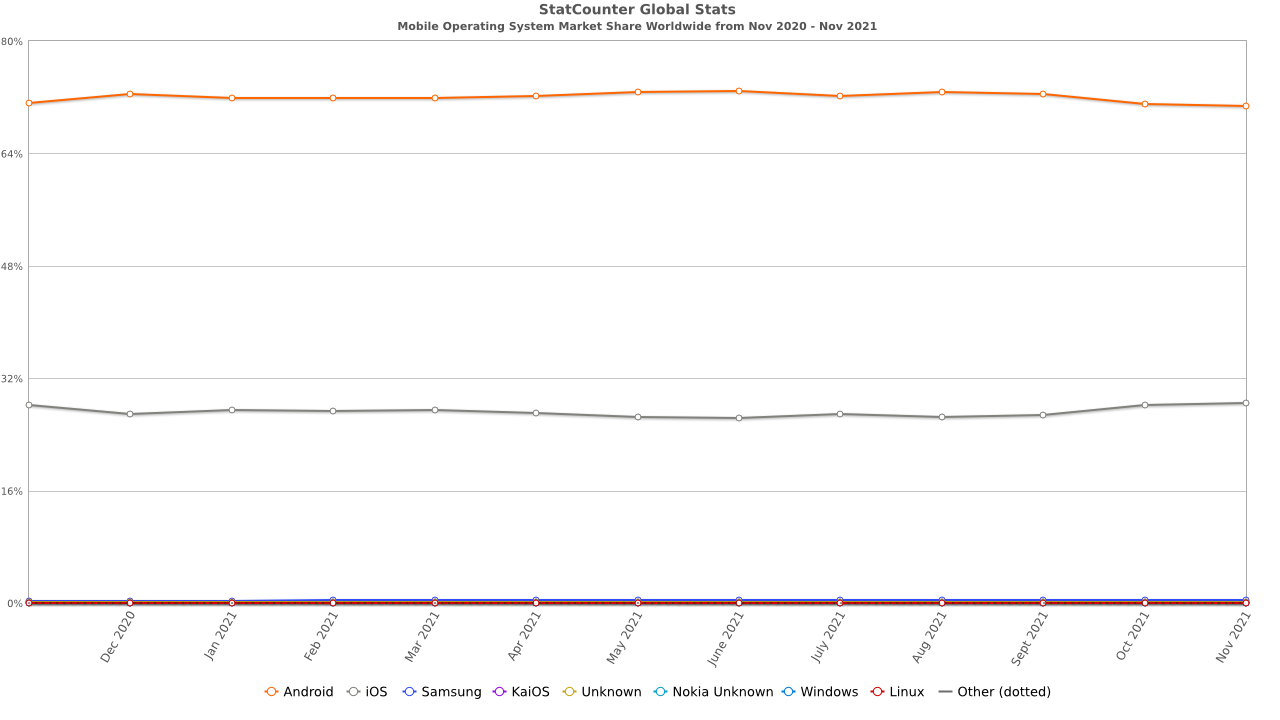
\includegraphics[width=10cm, angle=270]{Images/OS_market_share.png}
    \caption{Market share of mobile operating systems}
\end{figure}

\begin{itemize}
\item Native app: 
\end{itemize}

Native apps are apps developed in a language optimized for mobile devices. Currently, the market is divided into two platforms: Android and iOS. For Android development, the ability to handle Android SDK and Java-based Kotlin is necessary. For iOS development, the ability to handle Swift and a computer running Mac OS are necessary. The advantages of native app development are that it can maximize performance and that developers can take full advantage of the platform's features by calling and using the Native API. On the other hand, there are disadvantages in that you need to be familiar with handling the API of the platform and its low versatility due to it being platform-specific.

\begin{itemize}
\item  Web App:
\end{itemize}

Web apps are a combination of mobile web and native apps, and have the advantages of native apps while having the characteristics of mobile web. Like mobile web, web apps are developed with general web technology and run on mobile browsers, but they are characterized by high speed by adopting a single page method rather than a full browser method. The advantages of web apps are that there is no need to install a separate app, can be accessed from any browser on any device, and is easy to maintain. On the other hand, the disadvantages are that developers have to use only the browser API, not the platform API, it is difficult to execute, and the operation is not smooth.

\begin{itemize}
\item  Hybrid App:
\end{itemize}

A hybrid app is an app that blends the characteristics of a web app and a native app. The advantages of hybrid apps are that they can use both native APIs and browser APIs, so that various developments are possible, it is easy to develop because it is possible to develop an app with web development technology, and it can respond to multiple platforms with one development. On the other hand, the disadvantages are that you can use the native API only after learning native development knowledge, that you cannot increase the maximum performance because you run the app in the web view, and that the developer has to create the UI.\\

\item Choosing Native App - Android

\begin{itemize}
\item Native App:
\end{itemize}

This project will be implemented as an app to check and compare study time with other students, and save unknown words or incorrect questions. There is no reason to use the Native API to implement these functions. This is a function that can be implemented with just the browser API. However, it is appropriate to develop as a Native App from the beginning because there is a possibility of using the Native API in the future, such as using the Screen Time API to record study time, or using the mobile phone use control API to restrict the use of mobile phones during study.

\begin{figure}[htp]
    \centering
    
\includegraphics[width=8cm]{Images/android_pic.png}
    \caption{Overview on the three popular operating systems}
\end{figure}

\begin{itemize}
\item Android: 
\end{itemize}

There are two reasons to choose Android as the project platform. First, Android can have far more control over the phone than iOS does. Android is more capable to use powerful features that control lock screens and bring information about cell phone usage that iPhone cannot do. Secondly, there are team members who have experienced Android development. If this project has a leisurely development period, there is no big problem to take lectures from the beginning because there is enough time to build the foundation. However, in a situation where a month or two months is given, such as the current project, it is most important to bring out the maximum results in a way that each person can do well.

\begin{figure}[htp]
    \centering
    
\includegraphics[width=8cm]{Images/android.png}
    \caption{Android operating system}
\end{figure}

\end{enumerate}

\subsection{Choice of software development platform - NUGU Play Builder} 

\begin{figure}[htp]
    \centering
    
\includegraphics[width=8cm]{Images/nugu_inside.png}
    \caption{NUGU inside logo}
\end{figure}

NUGU Speaker will not be utilized alone in this project. NUGU Speaker will be used as a sub-device concept such as Apple Watch used with iPhone and Samsung Galaxy Watch used with Samsung Galaxy series smartphones.

\begin{enumerate}
\item Why using NUGU Speaker?
\begin{figure}[H]
    \centering
    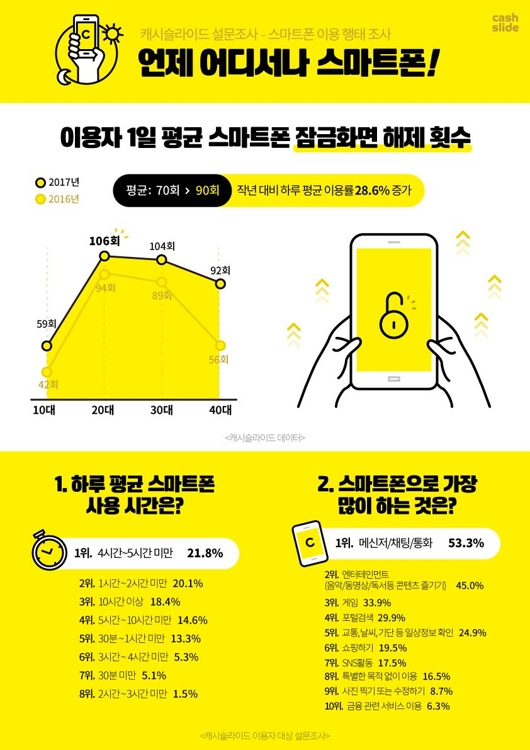
\includegraphics[width=8cm]{Images/why_nugu.png}
    \caption{Why to use NUGU Speaker?}
    \label{figure:useNuguSpeaker}
\end{figure}

The biggest problem when using academic applications is that students must use a smart phone. According to Fig. ~\ref{figure:useNuguSpeaker}, the top three items of the things that students do the most with your smartphone are things that interfere with their studies. The result tells that the more students use their phone, the more likely students are to do something other than study. Therefore, to use academic management applications such as Yeolpumta(열품타), students must be determined to never use content such as messengers, entertainment, and games. To overcome these shortcomings, it would be appropriate to use the NUGU speaker, which can minimize access to mobile phones, for learning recording.\\


\item How to use NUGU Speaker

\begin{itemize}
\item \textit{Recording Study Time:} Detailed settings including existing learning ability, personal information such as age and gender, and goal score setting are registered in advance with the smartphone application, and learning time is recorded with NUGU Speaker. The command is:

\begin{itemize}
\item Aria, Start study today
(아리야, 오늘 공부 시작) \\
 → start timer

\item Aria, breaktime
(아리야, 쉬는 시간) \\
→ pause timer

\item  Aria, Stop study today
(아리야, 오늘 공부 그만할래) \\
→ stop timer

\end{itemize}


\item \textit{Reading Wrong Answer Notes and Vocabulary:} According to an article in Health Chosun, \cite{b5} there is a study result that people can memorize the most efficiently if they study memorization subjects right before going to bed at night. If users record the wrong answer note picture and vocabulary not memorized properly through the mobile phone application, NUGU Speaker will read the information from the database and read it. The command is:

\begin{itemize}
\item Aria, Read wrong answer note
(아리야, 오답노트 읽어줘)  \\
→ start to read wrong answer note
\item Aria, Read vocabulary lists
(아리야, 단어장 읽어줘) \\
→ start to read vocabulary lists
\item Aria, Give me a vocabulary quiz
(아리야, 단어 퀴즈 내줘) \\
→ give a quiz from vocabulary lists randomly

\end{itemize}


\item \textit{Studying With Studymate:} A student can easily lose power when he(or she) studies alone. Best way to prevent this situation is to make a competitor. And our app, StudyBNB did it for you guys. We use study time data such as 'total\_study\_time' which represent average study time of a day in last week, and 'avg\_study\_time' which represent 'total\_study\_time' divided by number of studies that day. We find out some homogeneous groups in the users, and two people in these groups will be matched as a StudyMate. The command is:


 
\begin{itemize}
\item Aria, Tell me the information of my studymate
(아리야, 스터디메이트 정보 알려줘) \\
→ start to tell basic information of studymate
\item Aria, Is studymate studying now?
(아리야, 스터디메이트 지금 공부 중이야?) \\
→ start to tell whether studymate is studying now or not
\item Aria, Tell me the whole study time of my studymate
(아리야, 스터디메이트 오늘 공부시간 알려줘) \\
→ start to tell the study time of studymate

\end{itemize}

\end{itemize}


\end{enumerate}



\subsection{Choice of software development platform - Server} 

A server will be used for the NUGU AI speaker and Android app. The backend will be implemented with Firebase, and the database will be implemented with Firestore and Cloud Storage provided by Firebase. The server has a total of three roles. The first is the role of processing and storing user information recorded in the Android app. The second is the role of processing commands input from NUGU Speaker and return the result. Finally, it is the role of running commercial AI models on the server, such as an API that converts characters in an image into text, and an API that applies TTS to text.

\begin{enumerate}
\item Firebase

\begin{figure}[H]
    \centering
    
\includegraphics[width=8cm]{Images/firebase_logo.png}
    \caption{Firebase logo}
\end{figure}

Firebase is chosen because of its many advantages.
\begin{itemize}
\item It is free to access if Google account exists
\item The development speed is very fast because the backend work is standardized
\item Almost everything needed for development is provided
\item It is free to expand and contract server if paid option is chosen
\item Real-time monitoring of errors enables immediate feedback
\end{itemize}

Since a limited number of people have to take charge of parts such as Android app development, NUGU Play Builder, server and backend, and Dataset processing, a simple backend construction is prefered. In addition, it is appropriate to use Firebase because Firestore and Cloud Storage provided by Firebase were needed to proceed with the project.\\


\item Cloud Storage

\begin{figure}[H]
    \centering
    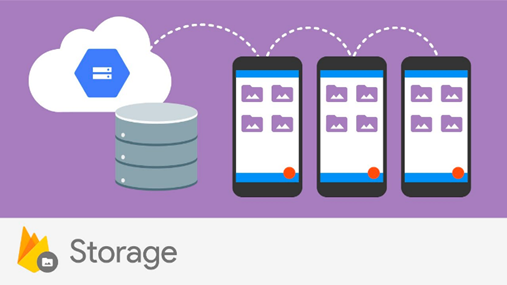
\includegraphics[width=8cm]{Images/fb_Cloud_storage.png}
    \caption{Firebase Cloud Storage}
\end{figure}

Cloud Storage is a database used to store large files such as images. It will serve to store the user's profile picture and a picture of the unknown word or incorrect question taken by the user with the smartphone.\\

\item Firestore

\begin{figure}[H]
    \centering
    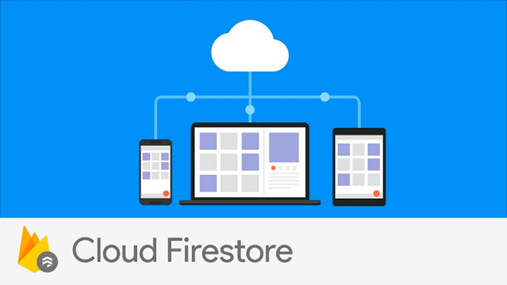
\includegraphics[width=8cm]{Images/fb_cloud_firestore.png}
    \caption{Firestore logo}
\end{figure}

Firestore is a NoSQL Database for mobile app development. It will be used to store users' information and learning time. Like chatting, there is a feature that users can share data in real time, and it will be a necessary function to build a system that can encourage competition for learning by sharing each other's learning time in real time.

\end{enumerate}



\subsection{Programming languages}

\begin{enumerate}
\item Kotlin

For the app development with Android Studio the language Kotlin is recommended. It's seamlessly integrated in the IDE and is the prefered language for developing Android apps according to Google. This makes it the clear choice for the app development.

\item Python

For working on machine learning capabilities like recommendation functions the language Python is recommended. Due to its simplicity and consistency, development is faster than other languages. Especially for machine learning, many libraries, and frameworks like NumPy and scikit-learn exist in Python. One disadvantage is the performance of the language compared to C or C++. For the recommendation function of ‘StudyBNB’, speed is not a relevant characteristic though.

\end{enumerate}

\subsection{Cost estimation}

The cost estimation for the development is provided below:

\begin{table}[H]
\caption{Cost Estimation}
\begin{center}
\begin{tabular}{|p{1.5cm}|p{4cm}|p{1cm}|}
\hline
\textbf{Resource} & \textbf{Description} & \textbf{Cost (KRW)} \\
\hline
Google Firebase	& Development platform and backend & 0 \\
\hline
Notion & Documentation and collaboration page & 0 \\
\hline
Jupyter Notebook & Coding environment for Python & 0 \\
\hline
Android Studio & IDE & 0 \\
\hline
Github & Code version control & 0\\
\hline
\end{tabular}
\end{center}
\end{table}


\subsection{Development environment}

For the development the following versions and resources are being used:

\begin{enumerate}
\item Computer:
\begin{itemize}
\item CPU: AMD Ryzen 7 4700U with Radeon Graphics 2.00 GHz
\item RAM: 16 GB
\item OS: Windows 10 Education Version 21H1
\end{itemize}

\item Android Studio:
\begin{itemize}
\item Version: Arctic Fox | 2020.3.1 Patch 3
\end{itemize}

\item Jupyter Notebook:
\begin{itemize}
\item Version: 6.3.0
\end{itemize}

\item Python: 
\begin{itemize}
\item Version: 3.8.8
\end{itemize}

\end{enumerate}



\subsection{Software in use}

An overview of existing software has been given in Chapter I.C. "Research on related software". Below is an detailed description on them and how StudyBNB wants to solve exisiting problems.

\begin{enumerate}
\item \textit{Yeolpumta(열품타)}

\begin{figure}[H]
    \centering
    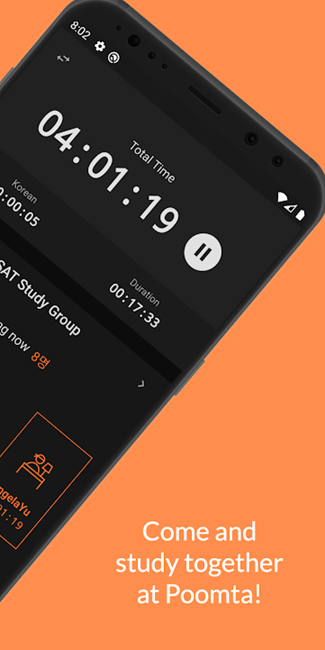
\includegraphics[width=4cm]{Images/Yeolpumta.png}
    \caption{Overview: 4.2 stars from 11,000 ratings and 1 Mio.+ downloads on Google Play Store}
\end{figure}

Yeolpumta is a widely popular study timer application in South Korea. Users can gather in study groups and see the rankings of each group member. It can prohibit its users running other apps while studying. It also allows users to focus by making a white noise if they want. Users can use the cam study function, where users can see the group members’ pictures, which are taken every 30 seconds. The video functions seem better, but they provide pictures only every 30 seconds because of cost issues. In addition, users can communicate with each other in a community.\\

\item \textit{Forest}

\begin{figure}[H]
    \centering
    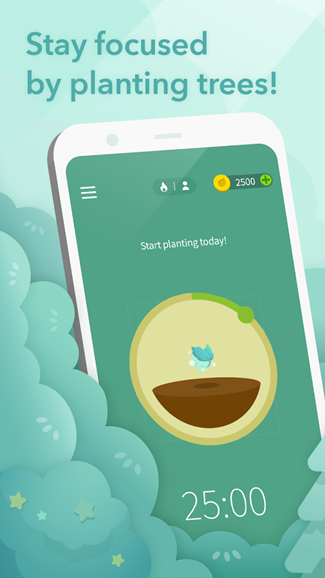
\includegraphics[width=4cm]{Images/Forest.png}
    \caption{Overview: 4.8 stars from 403,000+ ratings and 10 Mio.+ downloads on Google Play Store}
\end{figure}

In Europe, the app Forest is popular to focus on studying. While not using the phone, users can earn coins to exchange for planting a tree through a non-profit organization. Forest makes use of Gamification aspects to reward the user for not using the phone. There is a premium version which provides statistics and collaboration functions to challenge friends.\\

\item \textit{Focus To-Do: Pomodoro Timer}

\begin{figure}[H]
    \centering
    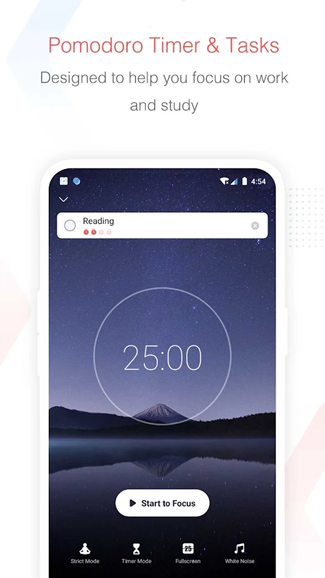
\includegraphics[width=4cm]{Images/FocusToDo.png}
    \caption{Overview: 4.7 stars from 157,000+ ratings and 1 Mio.+ downloads on Google Play Store}
\end{figure}

Focus To-Do: Pomodoro Timer is a study time checker that makes use of the pomodoro technique. Basically, the technique repeats a flow of 25 minutes of studying and 5 minutes of taking a break four times. After such a flow, the user takes a 30-minute break. This time management technique exists for many years since it has been proposed in the 1980s. This application also provides a white noise service and smartphone restriction mode.\\

\item \textit{Quanda}

\begin{figure}[H]
    \centering
    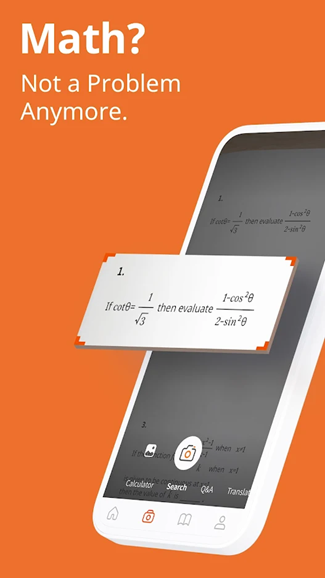
\includegraphics[width=4cm]{Images/Quanda.png}
    \caption{Overview: 4.1 stars from 447,000+ ratings and 10 Mio.+ downloads on Google Play Store}
\end{figure}

QANDA is an application that makes use of AI techniques such as optical character recognition (OCR) to provide appropriate answers to math questions. In case of needing more explanation, the user can contact tutors. The app also searches the web regarding given question so that users can study more about that type of problem.\\

\item \textit{AI TOEIC – RiiiD TUTOR}

\begin{figure}[H]
    \centering
    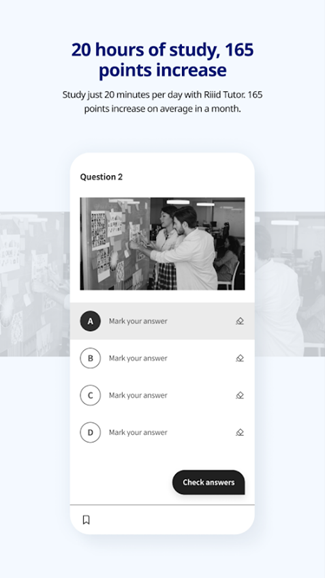
\includegraphics[width=4cm]{Images/AI_Toeic.png}
    \caption{Overview: 4.6 stars from 8,000+ ratings and 1 Mio.+ downloads on Google Play Store}
\end{figure}

RiiiD Tutor is an application that helps users study the English test TOEIC. The app is special since it uses AI techniques in analyzing users’ study data and recommends which parts to study for the test. It also enables personalized learning.\\

\item \textit{Conclusion}

In conclusion, all the mentioned apps are widely popular as displayed in the amount of ratings and downloads. Nevertheless, they have disadvantages that they are bound to the smartphone. This causes the learner to lose concentration by picking up the phone. Some apps also don't remind the learner of proper breaks. Another problem is that the user can't start other apps like QANDA or RiiiD Tutor to support the studies since it contradicts with the idea of the study apps.

This proposal plans to tackle these problems by combining an application with the smart speaker SKT NUGU to minimize smartphone usage.


\end{enumerate}


\subsection{Task distribution}

How we share our work is shown in the table below. Who will be in charge of what is determined by their experiences and abilities. However, if there are difficulties in each other's parts, we will help each other and proceed with the work.

\begin{table}[H]
\caption{Task Distribution}
\begin{center}
\begin{tabular}{|p{1.5cm}|p{5cm}|}
\hline
\textbf{Name} & \textbf{Task} \\
\hline
Useong Kim & 
\begin{itemize}
\item NUGU Play Builder
\item Database
\item Machine Learning
\item Documentation
\end{itemize}
 \\
\hline
Hankyu Park	& 
\begin{itemize}
\item NUGU Play Builder
\item Database
\item Machine Learning
\item Documentation
\end{itemize}
 \\
\hline
Dongjin Lim & 
\begin{itemize}
\item Backend
\item Project Management
\end{itemize}
 \\
\hline
Sangyun Chi	& 
\begin{itemize}
\item UI Design
\item Application
\item Documentation
\end{itemize}
 \\
\hline
Michael Sklors & 
\begin{itemize}
\item UI Design
\item Application
\item Documentation
\end{itemize}
\\
\hline
\end{tabular}
\end{center}
\end{table}


\section{Specifications}

This chapter describes required specifications of the app that aim to fulfil the requirements of Chapter II. Several drafts for different screen in the app should give an idea on how the final version could look like.

\subsection{Splash Page}

\begin{figure}[htp]
    \centering
    
\includegraphics[width=4cm]{Images/Splash_page.png}
    \caption{Splash page}
\end{figure}

The splash screen is a graphic element consisting of a window containing an image, logo, and the current version of the software. It is displayed for about 0.5 second to avoid showing a blank screen during the loading time of the app's data. It also serves to express the brand identity of the 'StudyBNB'.

\subsection{Login Function}

\begin{figure}[htp]
    \centering
    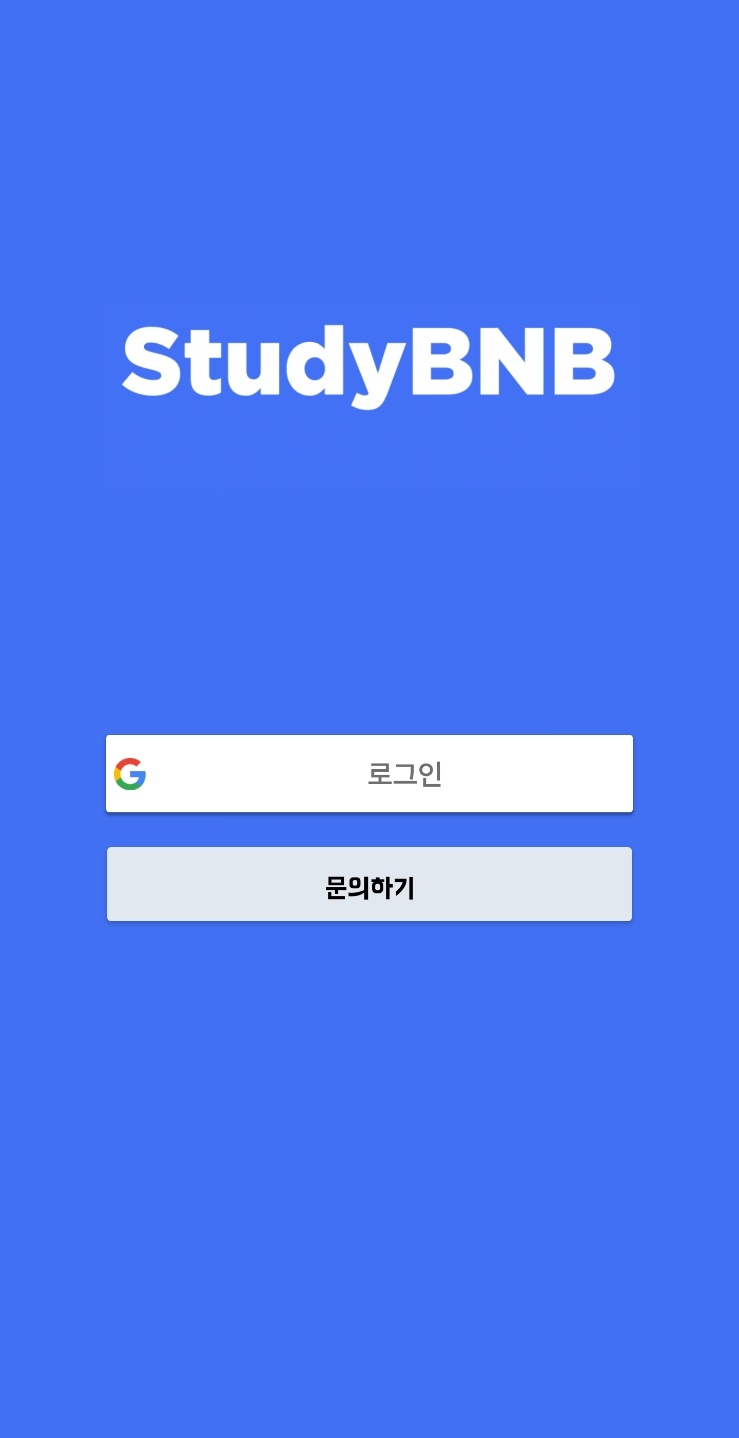
\includegraphics[width=4cm]{Images/App_Login_page.png}
    \caption{Login page}
\end{figure}

\begin{enumerate}
\item Authentification : Firebase uses various authentication methods such as email/password, phone, Google, play games, Facebook, Twitter, and GitHub.
\begin{itemize}
\item Click "Google Login" and if the key value authenticated, "Login Success" message appears.
\item If the key value is not established, pop-up message indicating that login failed.
\item If the login is successful, the main page appears.
\end{itemize}

\item Contact : If there is a problem with logging in, users contact the product manager and developer.
\begin{itemize}
\item Click "Contact" button, a little dialog will pop up that users can report the errors.
\item Errors written by the user are sent to the developer's mail.
\end{itemize}
\end{enumerate}

\subsection{Main Page}

\begin{figure}[htp]
    \centering
    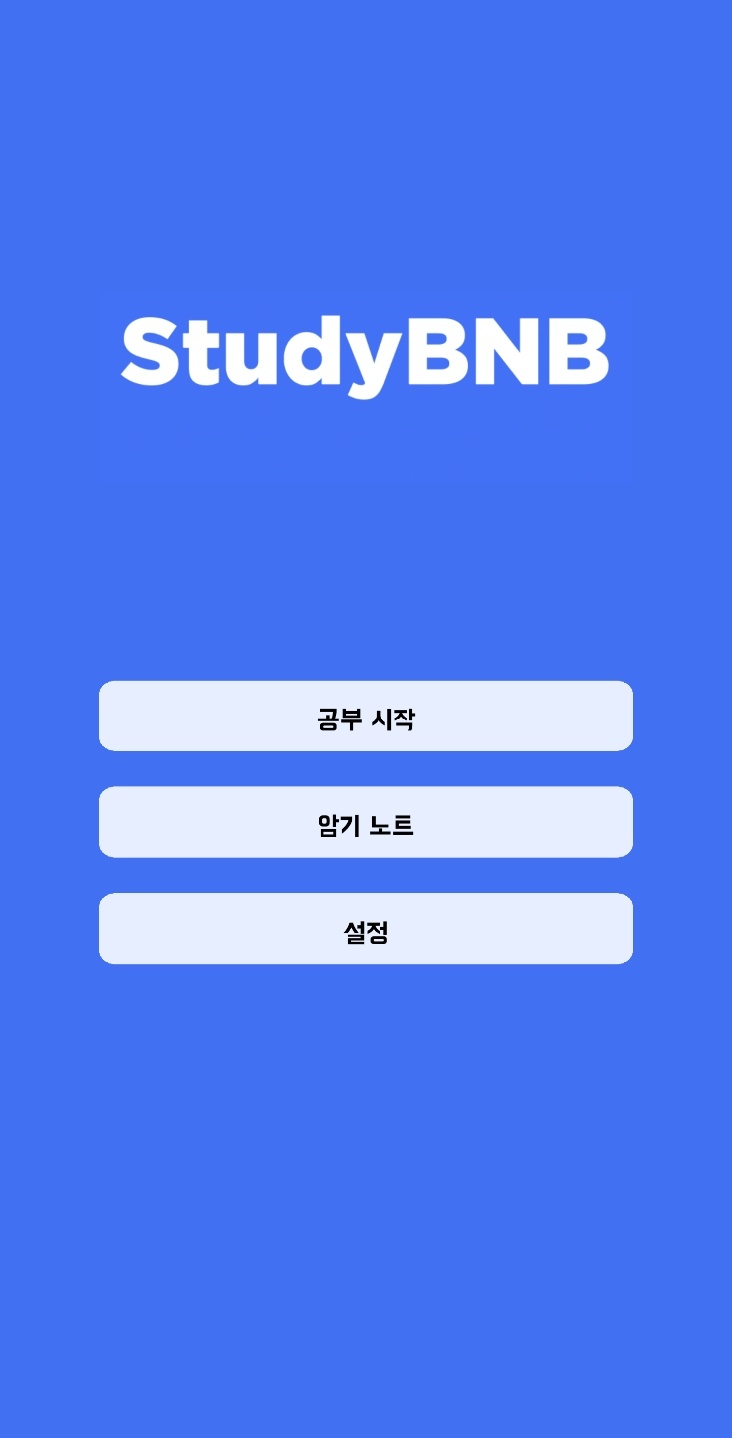
\includegraphics[width=4cm]{Images/app_main_page.png}
    \caption{Main page}
\end{figure}

When the user logs in successfully, Main screen appears. Main screen is visible only when users logged in.

\begin{enumerate}
    \item Timer : When the users click 'timer' icon on the main screen, the main screen will change into timer page screen. It will be shown only when users are log-in state.
    
    \begin{itemize}
        \item A logged-in user can start a timer by requesting to NUGU speaker and measure the study time.
        \item When a user wants to take a break or finish studying, the timer can be stopped by requesting to the speaker.
    \end{itemize}
    
    \item My Note : If the user click 'My note' icon on the main screen, the main screen will change into 'My note view page’.
    
    \begin{itemize}
        \item A logged-in user can note their own answer to memorize or words that they did not know before.
    \end{itemize}
    
    \item Settings: When the users click 'settings' icon on the main screen, the main screen will change into 'Settings page'
    
    \begin{itemize}
        \item Users can delete one's account or log out in Settings page.
    \end{itemize}
    
\end{enumerate}


\subsection{My Note-taking page}

\begin{figure}[htp]
    \centering
    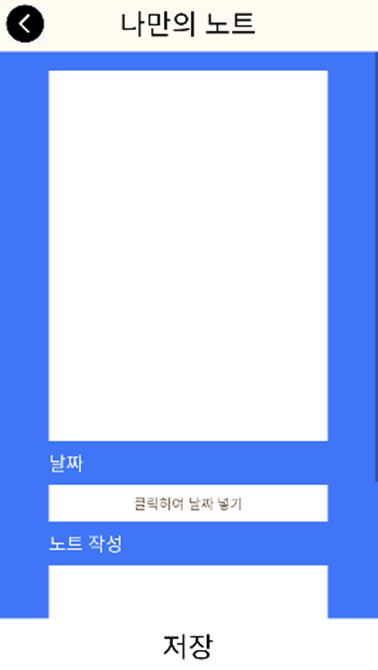
\includegraphics[width=4cm]{Images/app_notetaking_spec.png}
    \caption{Note-taking page}
\end{figure}

The 'My note-taking page' consists of box to insert a photo, a field for date and field for writing notes.

\begin{enumerate}
    \item Inserting a photo : When a user encounters an unknown problem or word, it can be recorded in the form of photo
    \item Recording the date : Users can record the date when the note was saved.
    \begin{itemize}
        \item Problems that were previously wrong or unknown can also be recorded from an earlier date.
    \end{itemize}
\end{enumerate}


\section{Architecture Design and Implementation}

\subsection{Overall Architecture}

\begin{figure}[H]
    \centering
    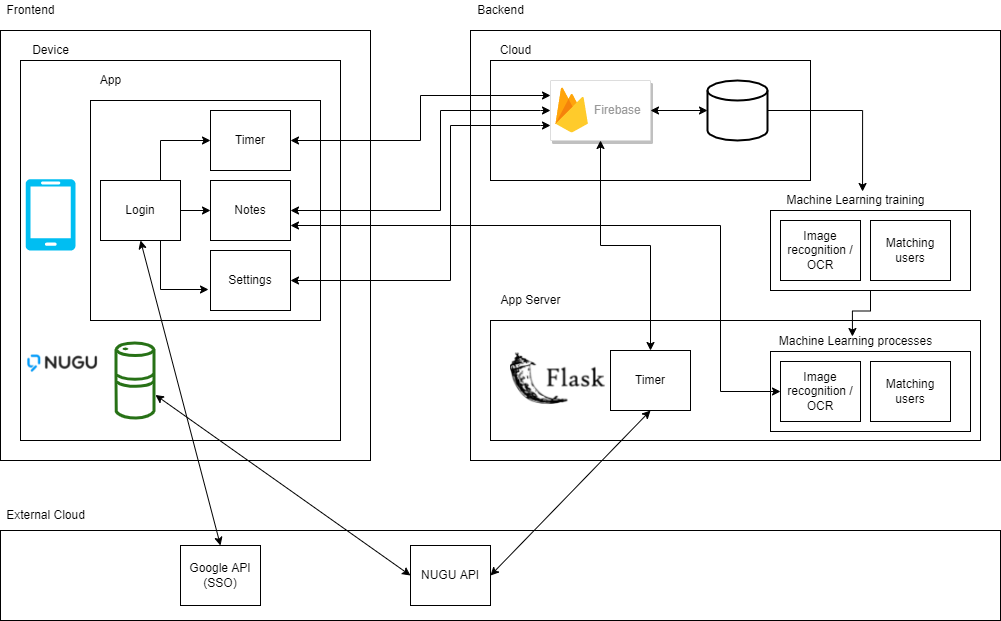
\includegraphics[width=12cm, angle=270]{Images/architecture_studybnb.png}
    \caption{StudyBNB Architecture}
    \label{figure:architecture}
\end{figure}

Fig. ~\ref{figure:architecture} displays that StudyBNB consists of three parts: Frontend, Backend and external Cloud. The frontend focuses on the visual elements of the app that the user interacts with while the backend focuses on the server side that the user can't see. The external cloud provides interaction with external services.

Frontend is represented by the mobile app and the NUGU speaker. The former one allows interaction with the modules "login", "timer", "notes" and "settings". The "login" function makes use of Google sign-in and communicates with the Google API. NUGU Speaker needs to work with the NUGU API to use functions of the mobile app.

Backend is represented by the cloud consisting of the backend capabilities of Firebase and its Firestore database. The functions from the frontend save and retrieve data in Firebase. Another part of the backend is the app server which is built on the Python web-framework Flask. The app server has a timer function that uses words from the NUGU speaker and data from Firebase as input and starts the timer. For machine learning capabilities, data from the Firestore database is used to train the model for image recognition and matching users capabilities. Inside the app server the model will be applied for the notes function.


\subsection{Directory Organization}

\begin{table}[H]
\caption{Directory Organization}
\begin{center}
\begin{tabular}{|p{2cm}|p{2.5cm}|p{2cm}|}
\hline
\textbf{Directory} & \textbf{File names} & \textbf{Module names in use} \\
\hline
studybnb/app/main &	InfoActivity.kt
LoginActivity.kt
MainActivity.kt
NoteListActivity.kt
NoteWriteActivity.kt
SettingActivity.kt
SplashActivity.kt
SubjectActivity.kt
TimerActivity.kt & 
\begin{itemize}
\item App
\item Google API
\item Firebase
\item Image recognition / OCR
\end{itemize}
 \\
\hline
studybnb/app/
main/model & StudyTimerModel.kt
UserInfoModel.kt & 
\begin{itemize}
\item Timer
\item Notes
\item Settings
\end{itemize}
 \\
\hline
studybnb/app/
res/drawable &	back.png
studybnb.png &	App
 \\
\hline
studybnb/app/
res/layout & activity\_info.xml
activity\_login.xml
activity\_main.xml
activity\_note\_list.xml
activity\_note\_write.xml
activity\_setting.xml
activity\_splash.xml
activity\_subject.xml
activity\_timer.xml & 
\begin{itemize}
\item App
\item Google API
\end{itemize}
 \\
\hline
ai & kmean.py &	
\begin{itemize}
\item Machine Learning Training
\item Machine Learning Processes
\end{itemize}
\\
\hline
ai/data	& csv\_data\_example.csv &	
\begin{itemize}
\item Machine Learning Training
\item Machine Learning Processes
\item Database
\end{itemize}
\\
\hline
flask &	app.py
firebase.json &	
\begin{itemize}
\item NUGU API
\item Firebase
\item App Server/Timer
\end{itemize}
\\
\hline
documentation &	Documentation.docx
Documentation.pdf & Documentation
\\
\hline
\end{tabular}
\end{center}
\end{table}

\subsection{Module 1: Frontend}

\begin{enumerate}
    \item Login
    \begin{enumerate}
        \item Purpose: The login module represents secure user management
        \item Functionality: Through Single-Sign-On with the Google API, the user can login to StudyBNB. In case of issues the user can use the report button to send an email with predefined text to the admin team.
        \item Class Components: LoginActivity
    \end{enumerate}
    
    \item Main
    \begin{enumerate}
        \item Purpose: Main page to navigate to the functions of StudyBNB
        \item Functionality: The user can choose from three buttons. The first one leads to timer function, second one to note taking function and third one to setting function.
        \item Class Components : MainActivity
    \end{enumerate}
    
    \item Timer
    \begin{enumerate}
        \item Purpose: Being able to record studying times to get insights to studying habits
        \item Functionality: First, the user chooses a subject from the predefined buttons. After that, the user gets led to the timer page. There he can start the timer and finish it. After starting the timer, a new entry to the database will be created.
        \item Class Components: TimerActivity, SubjectActivity
    \end{enumerate}
    
    \item Notes
    \begin{enumerate}
        \item Purpose: Being able to take notes for a subject and save them in the app
        \item Functionality: Same as in Timer, the user chooses a subject first. After that, the user can choose from a list of existing notes or create a new one. When creating a new one, the user can upload a picture and write text for the note.
        \item Class Components: NoteWriteActivity
    \end{enumerate}
    
    \item Settings
    \begin{enumerate}
        \item Purpose: User management to log off or delete user
        \item Functionality: Users can change settings of the application and their basic information.
        \item Class Components: SettingsActivity
    \end{enumerate}
\end{enumerate}

\subsection{Module 2: External Cloud}

\begin{enumerate}
    \item Google API (SSO)
    \begin{enumerate}
        \item Purpose: Convenient and state-of-the-art login functionalities for the user
        \item Functionality: By using the Google API, the user can login with his Google account to login to StudyBNB. 
    \end{enumerate}
    
    \item NUGU API
    \begin{enumerate}
        \item Purpose: Providing NLP functionalities to transform spoken words to functions in StudyBNB
        \item Functionality: Through pre-defined intents and actions in the NUGU Play Kit the NUGU speaker can understand sentences and execute actions in the app server.
    \end{enumerate}
\end{enumerate}

\subsection{Module 3: Backend}

\begin{enumerate}
    \item Firebase
    \begin{enumerate}
        \item Purpose: Backend capabilities and database.
        \item Functionality: The Firestore Database stores data from the app or the NUGU actions in collections. Collections consist of Documents, while those consists of fields. New entries are done in documents and fields can be updated.
    \end{enumerate}
    
    \item App Server
    \begin{enumerate}
        \item Purpose: Backend capabilities for NUGU speaker, StudyBNB functions and machine learning processes
        \item Functionality: When receiving actions from the NUGU API, the app server uses internal functions to start or stop the timer. The data gets updated in Firebase.
    \end{enumerate}
    
    \item Machine Learning Training
    \begin{enumerate}
        \item Purpose: Training a machine learning model based on a dataset
        \item Functionality: The Firestore Database and a dedicated dataset serve as a basis. A k-means clustering algorithm as unsupervised learning will be used.
    \end{enumerate}
    
    \item Machine Learning Processes
    \begin{enumerate}
        \item Purpose: Using machine learning model in app / NUGU actions functionalities
        \item Functionality: The trained model will be run and the results will be used for functions.
    \end{enumerate}
    
\end{enumerate}

\section{Use Cases}

\subsection{Use Case 1 - Android Application}

\begin{enumerate}
    \item Use Case Diagram
    
    \begin{figure}[H]
    \centering
    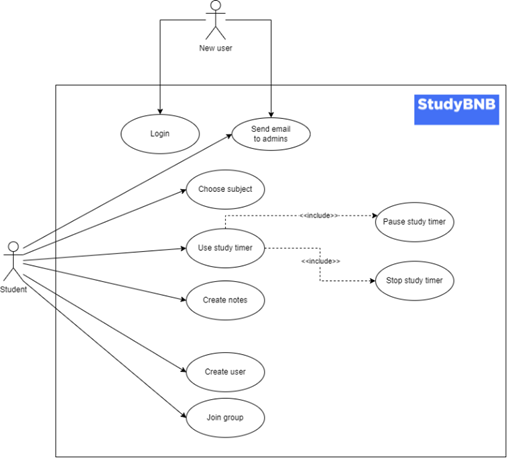
\includegraphics[width=8cm]{Images/use_case_diagramm.png}
    \caption{Use Case Diagram for the app}
\end{figure}

The use case diagram displays two actors: A "new user" and a "student". The new user only has use cases to login to the StudyBNB app or send an email to admins.

When logged it, the new user will be a in the role of student and can access the functions of the StudyBNB service. In case of deleting the user, the student will be back in the role of a "new user".\\

\item Main Functions

\begin{enumerate}
    \item \textit{Login / Send email to admins}
    
    \begin{figure}[htp]
    \centering
    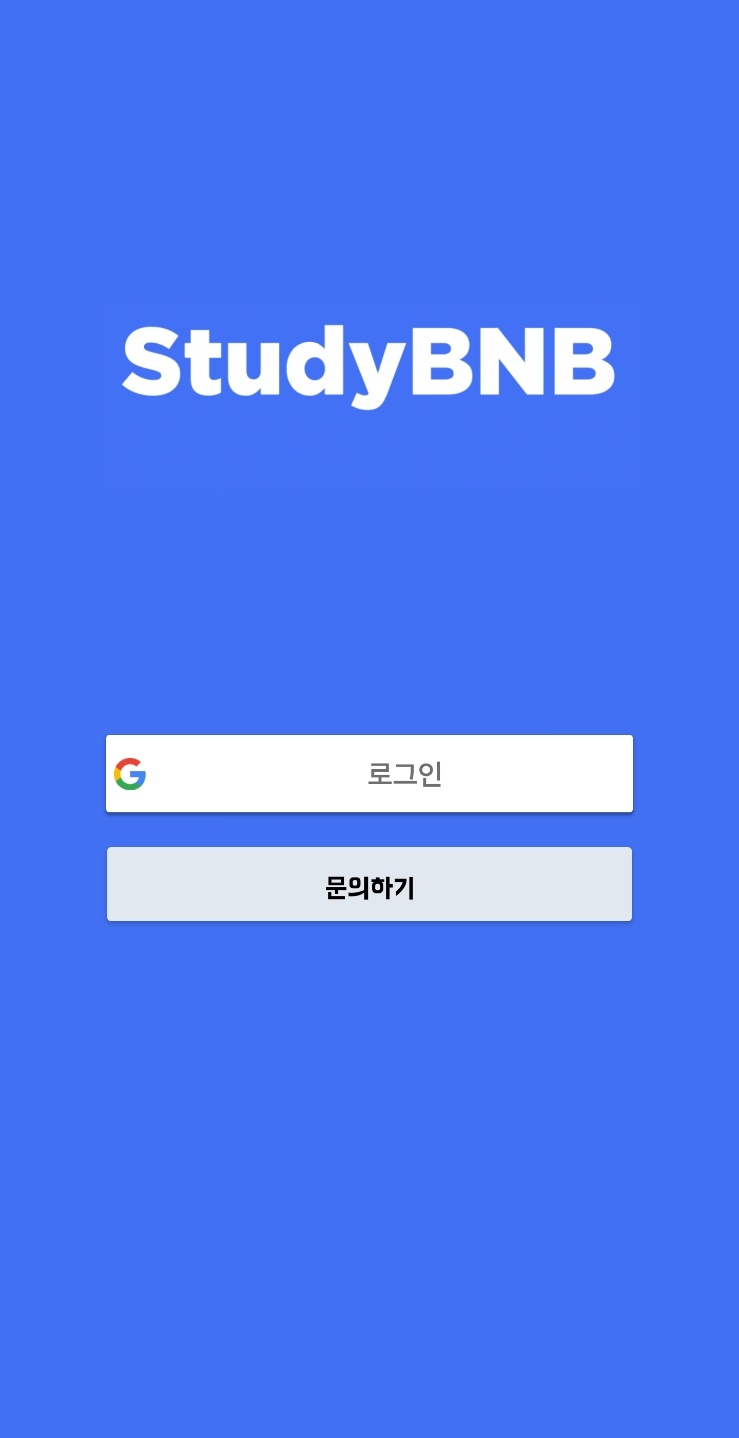
\includegraphics[width=5cm]{Images/App_Login_page.png}
    \caption{Login page}
    \label{figure:loginPage}
\end{figure}

    When opening the app, the user lands on the login page as in Fig. ~\ref{figure:loginPage} . Here he can choose between two buttons: Sign In via Google or "문의하기" / "Ask".
    
    As a new user, the first button opens a "Google account" dialogue which requires the user to enter his credentials. After using the login function once, the StudyBNB app remembers the user and he can enter the next screen just by pressing the button.

    \begin{figure}[htp]
    \centering
    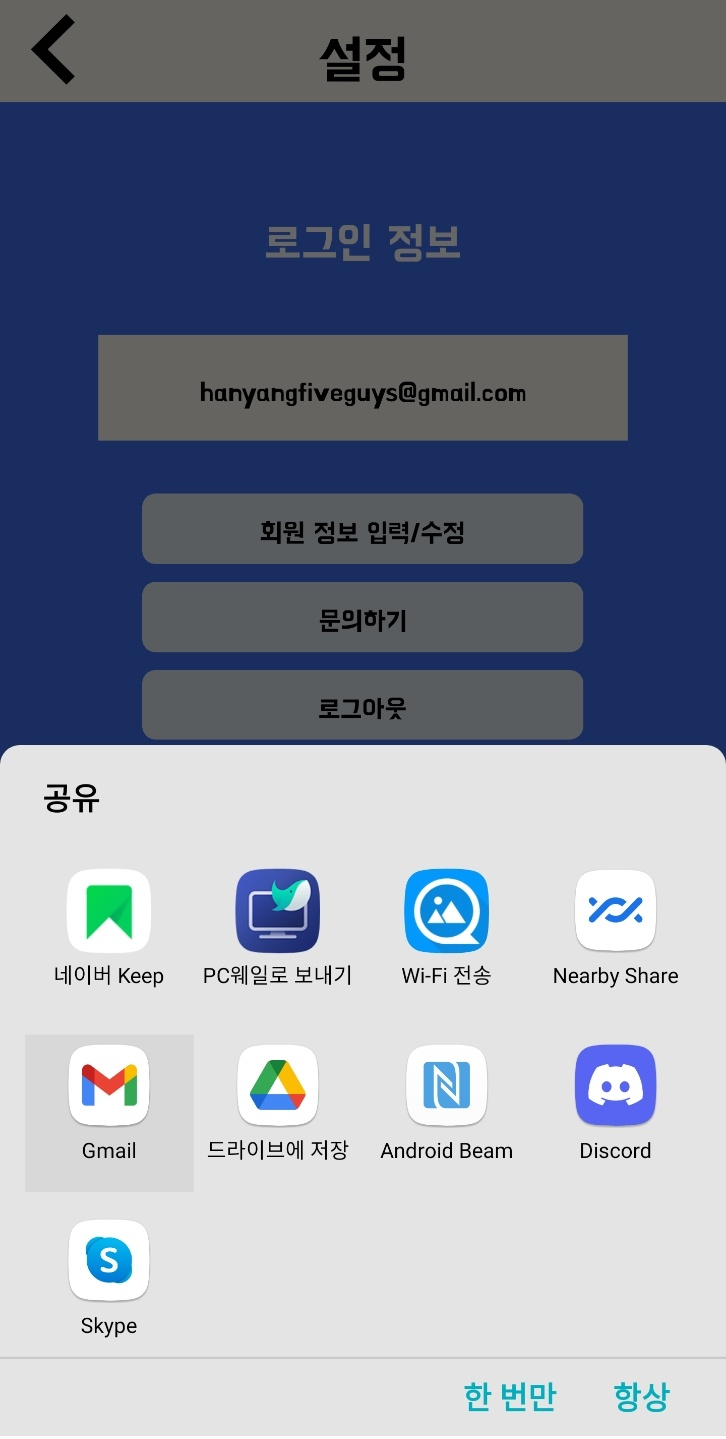
\includegraphics[width=5cm]{Images/app_send_email.png}
    \caption{Send email option}
    \label{figure:sendEmailPage}
\end{figure}
    

    


In case of inquiries or issues, the user can use the second button. It opens the prefered email app of the user and prepares a pre-defined email for the admin team as in Fig. ~\ref{figure:sendEmailPage}.

This function fulfills the requirements F1) User Management, N1) Security, N6) Usability by offering a basic account management and keeping the data private.\\
    
    \item \textit{Create user / Join group}
        
        \begin{figure}[htp]
    \centering
    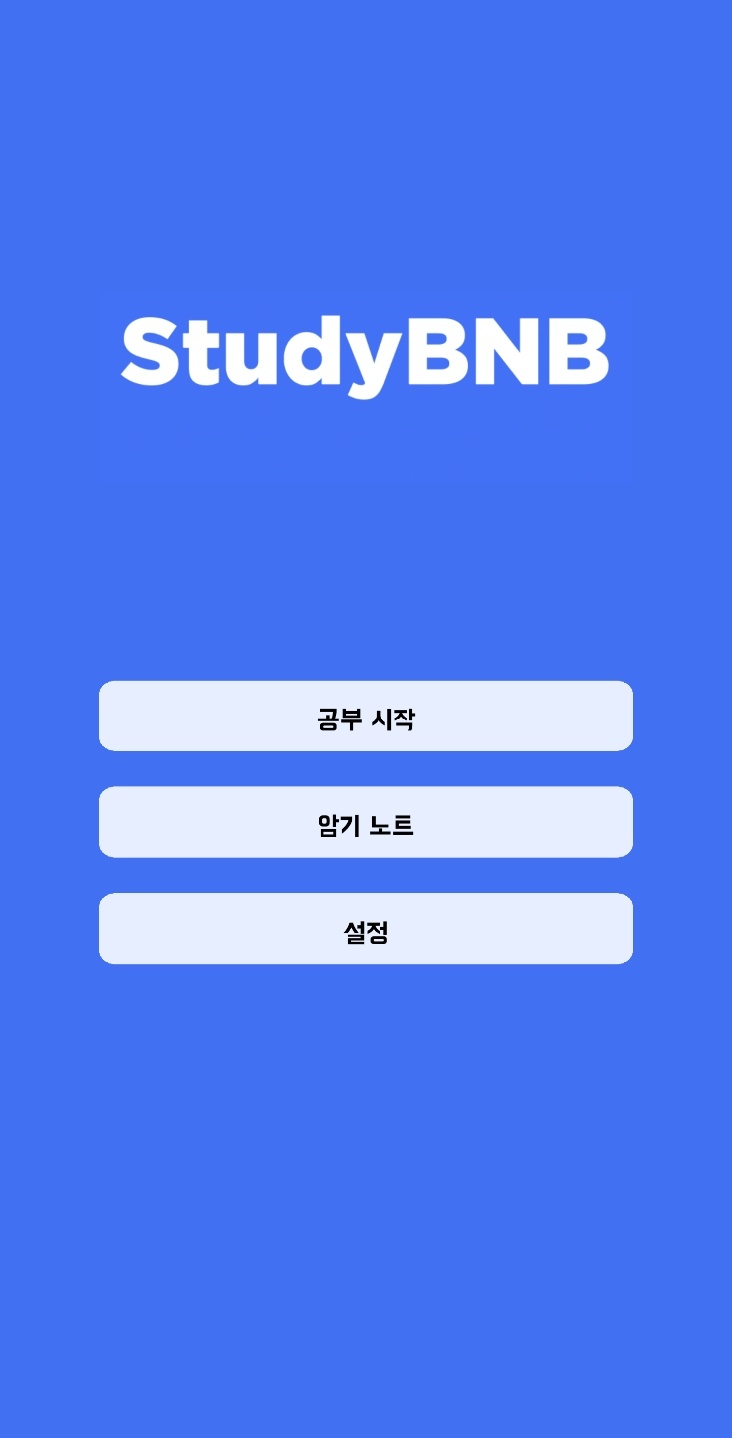
\includegraphics[width=5cm]{Images/app_main_page.png}
    \caption{Main page}
    \label{figure:mainPage}
\end{figure}
    
    After logging in, the user always starts at the Main screen as in Fig. ~\ref{figure:mainPage}. In the third button "설정"/"Setting" he can enter the settings screen.
    
    \begin{figure}[htp]
    \centering
    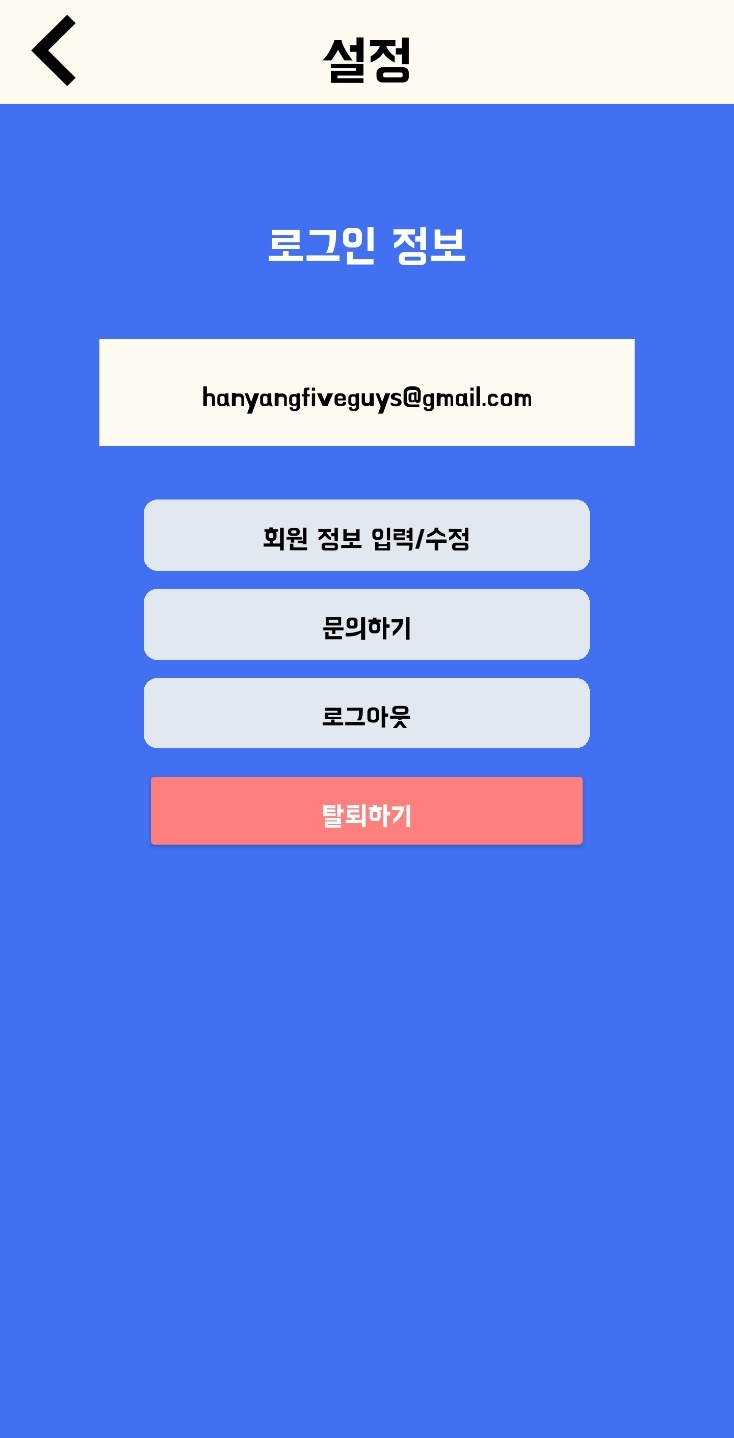
\includegraphics[width=5cm]{Images/app_settings.png}
    \caption{Settings page}
\end{figure}

The settings screen is an overview over 로그인 정보/Login information. The white label at the top displays the email that is used for login.

Button 1 is 회원정보 입력/수정 or Enter/Modify membership information.

Button 2 is 문의하기/Contact which works like in the Login page.

Button 3 is 로그아웃/Sign out which signs out the user from the app and brings him back to the login page.

Button 4 is 탈퇴하기/Leave the group which removes the personal data of the membership information and login information. A dialog requests the user to confirm his decision.


        \begin{figure}[htp]
    \centering
    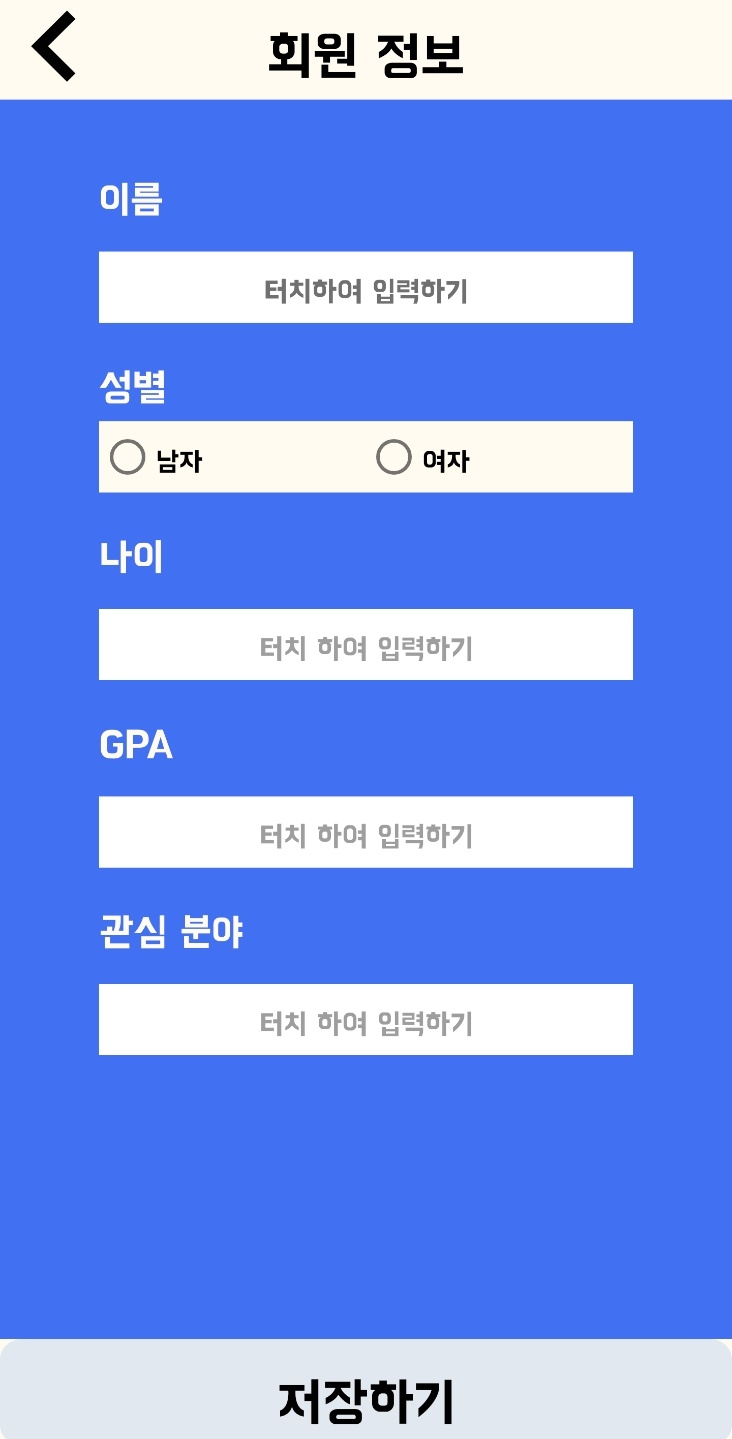
\includegraphics[width=5cm]{Images/app_userSetting.png}
    \caption{User settings page}
\end{figure}
    
    After clicking the first button, the user lands in the page to enter or edit his membership information. There he can enter his name, gender, age, GPA and interests. The button "저장하기" saves the entered values.

This function fulfils the requirements F1) User Management, F2) Creating a Study Group, N1) Security by allowing the user manage data about himself and delete it for privacy reasons.

It partly fulfils the requirement 4) Information Sharing Function (about study time) by giving insights about characteristics from the student but he can't see it from other group members.\\

    
    \item \textit{Start study timer}
    
        \begin{figure}[htp]
    \centering
    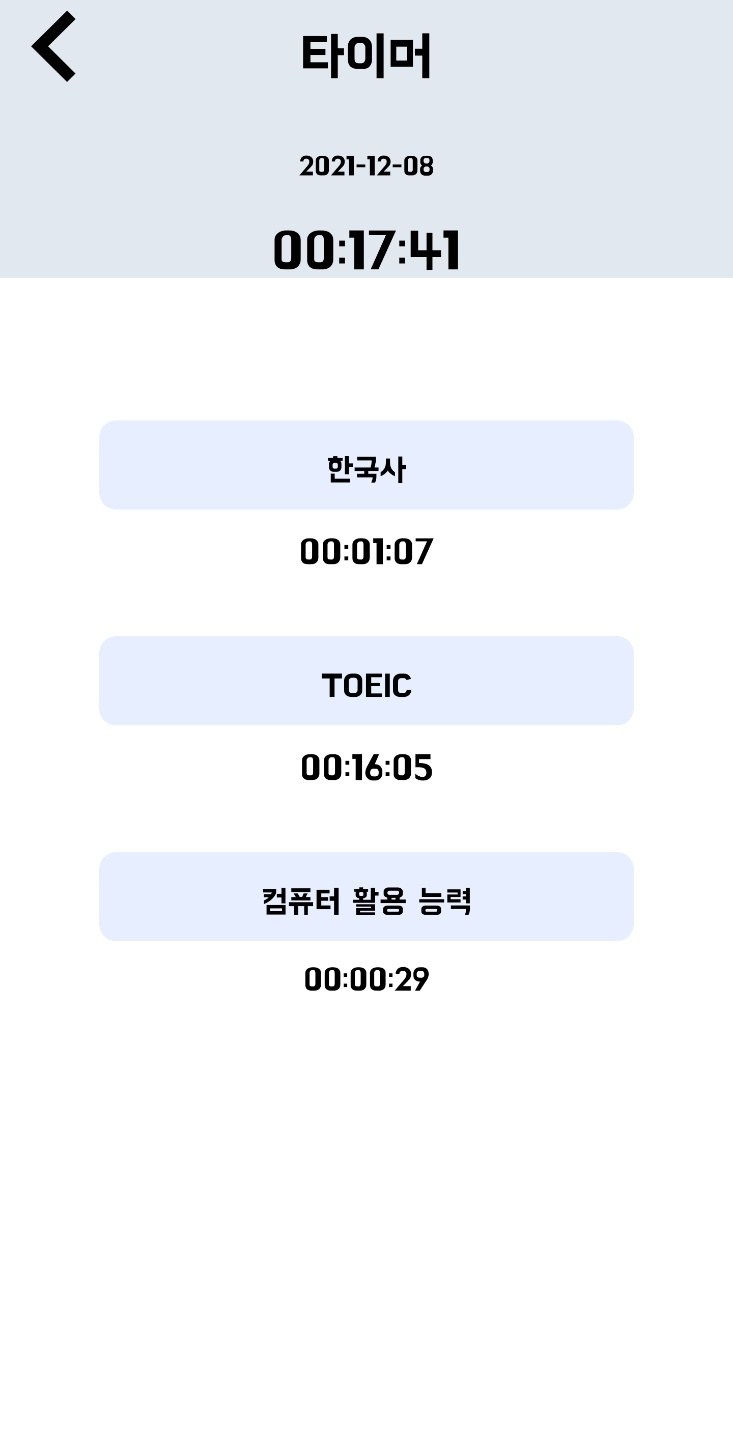
\includegraphics[width=5cm]{Images/app_timer_overview.png}
    \caption{Timer overview page}
\end{figure}

When clicking the first button on the main page, the user gets led to the subject page. He can choose from the three subjects "History", "TOEIC" and "Computer Specialist" with each displaying accumulated study time of the day. Clicking a button leads the user to the timer function.

    \begin{figure}[htp]
    \centering
    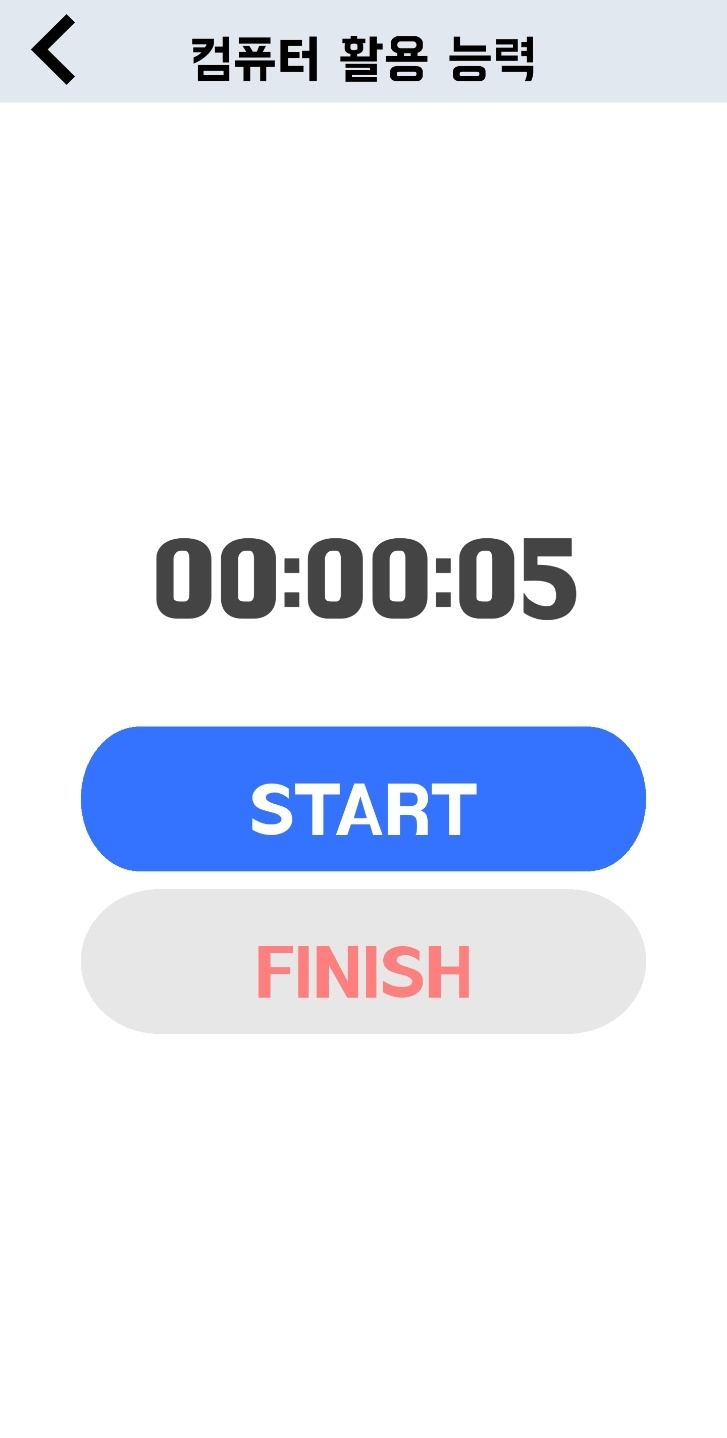
\includegraphics[width=5cm]{Images/app_start_timer.png}
    \caption{Timer page}
\end{figure}

The timer page contains an overview on the current subject and the timer itself. Clicking the start button starts the timer.

This function fulfils the requirements F3) Timer Function, N3) Performance, N6) Usability by allowing a quick and convenient usage of a study timer.\\

    
    \item \textit{Stop study timer}
    
\begin{figure}[H]
    \centering
    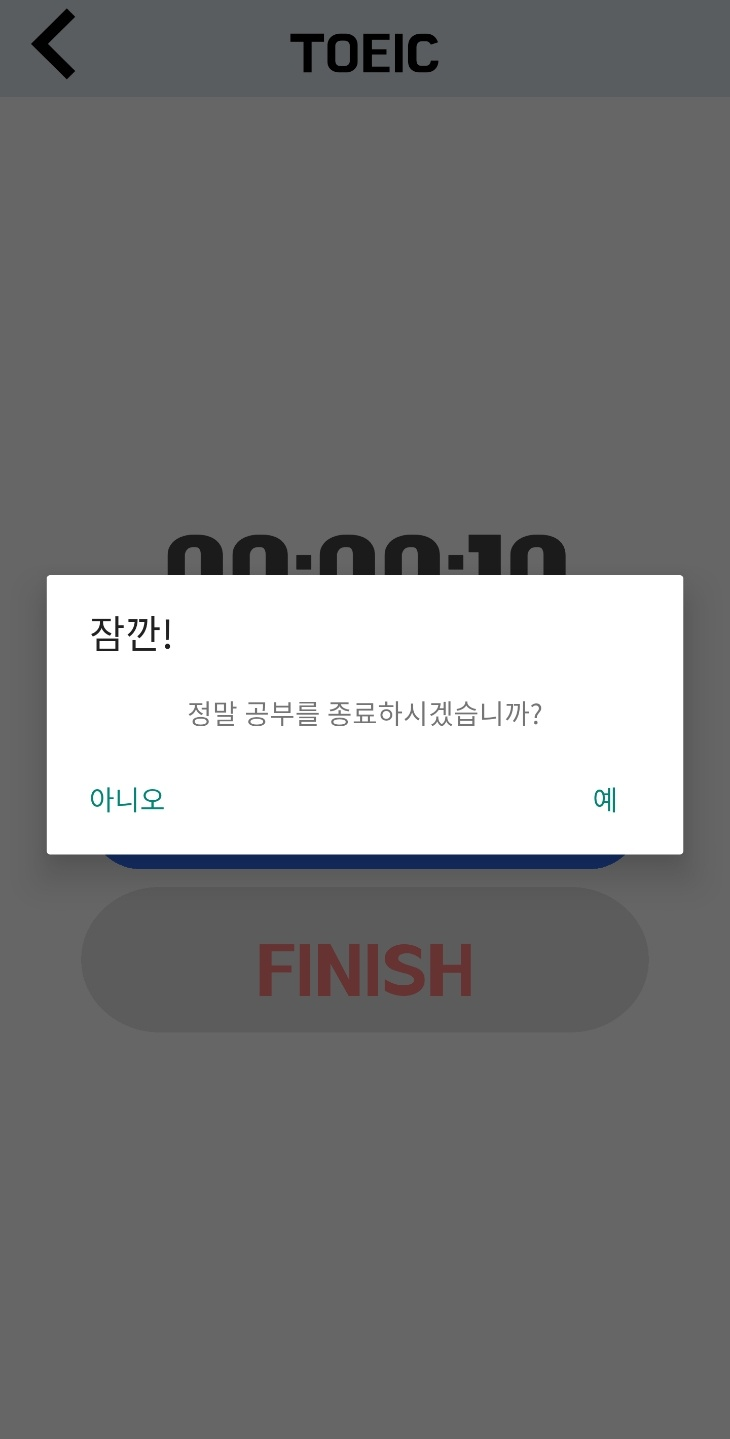
\includegraphics[width=5cm]{Images/app_stop_timer2.png}
    \caption{Dialog to stop timer}
\end{figure}

When the user is done studying, he can press the "Finish" button. It opens a dialogue to confirm that he wants to stop the timer. When clicking "Yes", he gets sent back to the main page.


        \begin{figure}[htp]
    \centering
    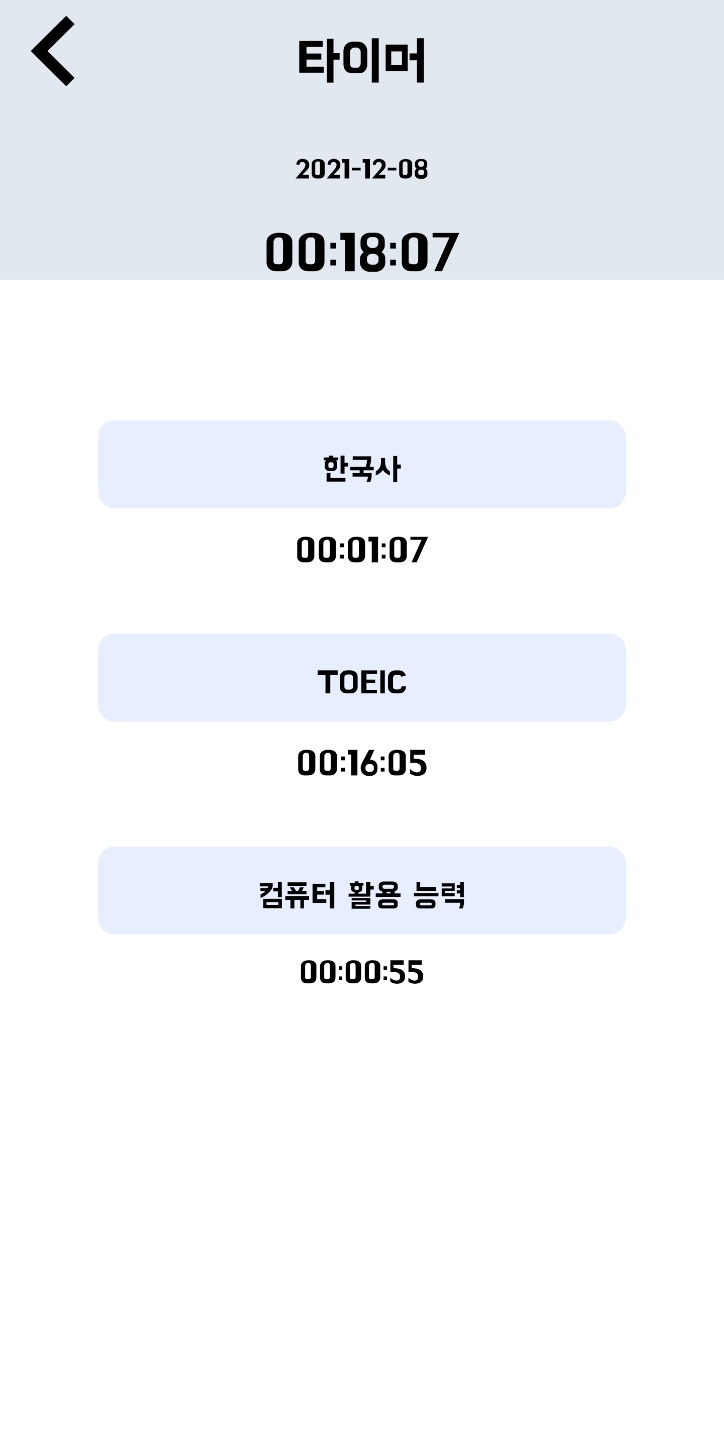
\includegraphics[width=5cm]{Images/app_stop_timer.png}
    \caption{Result after stopping timer}
\end{figure}

In the background, the duration of studying is saved. When entering the timer again, he can see that the accumulated study time has increased by the previous study block.

This function partly fulfils the requirements F4) Information Sharing Function (about study time), 5) Group Ranking and 6) Feedback. The information about the studying time, subjects and current status of studying is being saved but he can only compare his studying style by looking at the data in the backend.\\
    
    \item \textit{Create notes}
    
            \begin{figure}[htp]
    \centering
    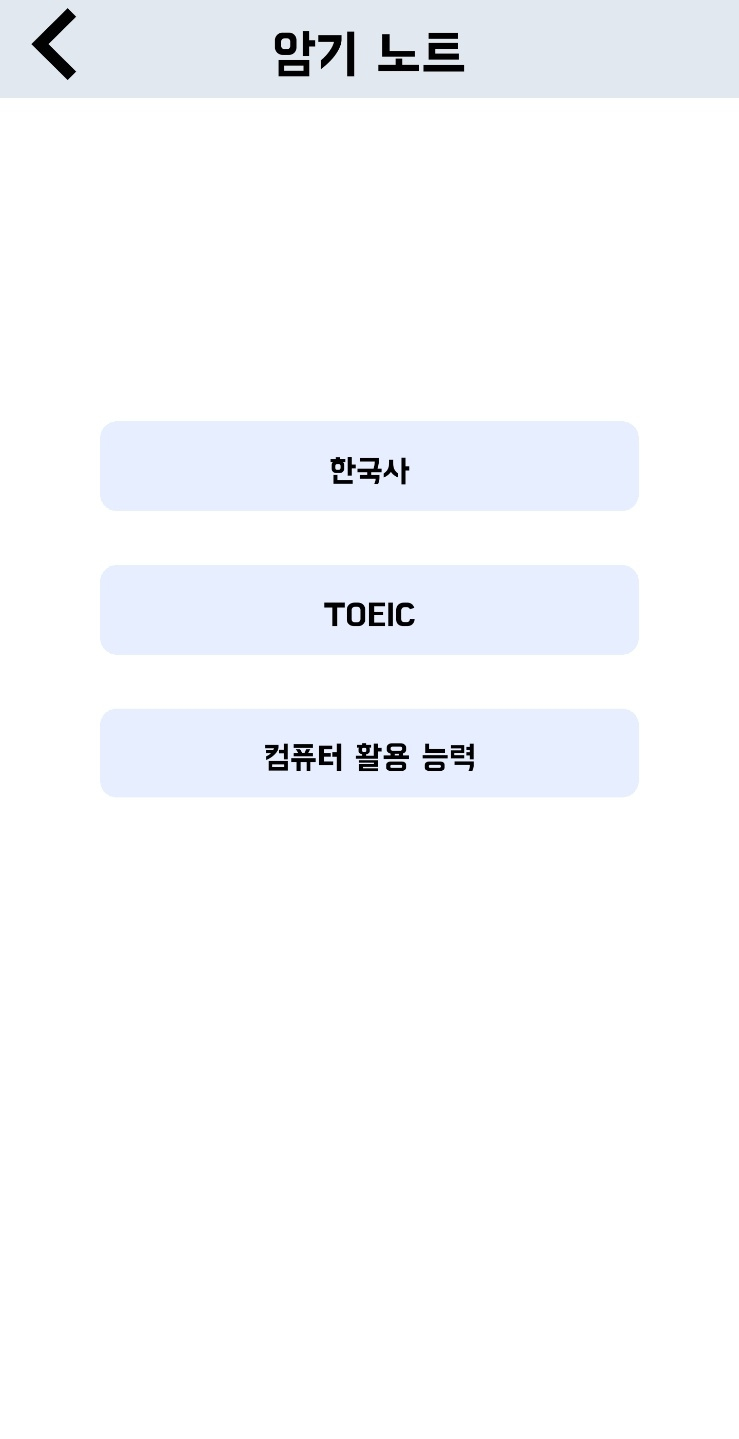
\includegraphics[width=5cm]{Images/app_note_subjects.png}
    \caption{Choosing subjects for notes}
\end{figure}

When the user clicks on the second button in the main screen, he needs to choose a subject just like with the timer. After choosing a subject to study, he gets let to an overview page of existing notes. In case no note exist, he can click at the blue button at the buttom to create a new note.

        \begin{figure}[htp]
    \centering
    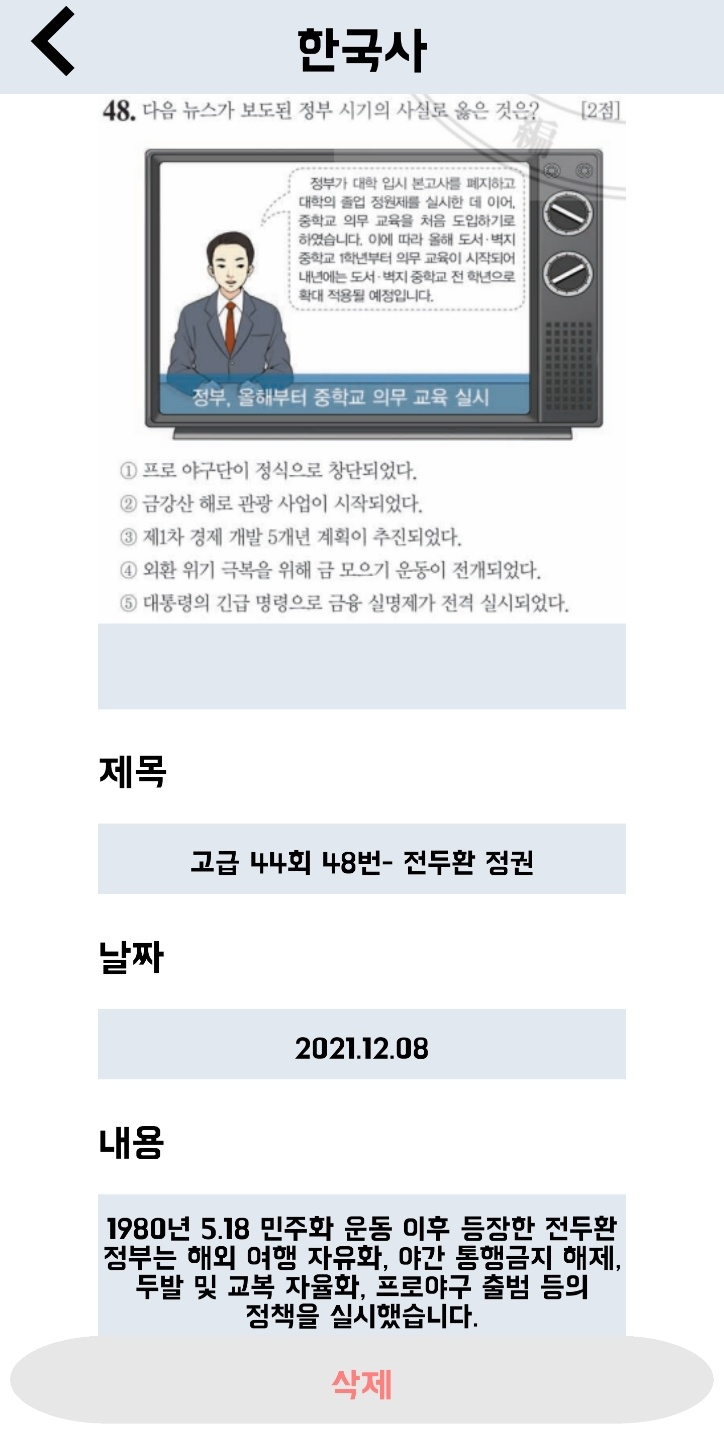
\includegraphics[width=5cm]{Images/app_note_history.png}
    \caption{Create a note for history subject}
\end{figure}

        \begin{figure}[htp]
    \centering
    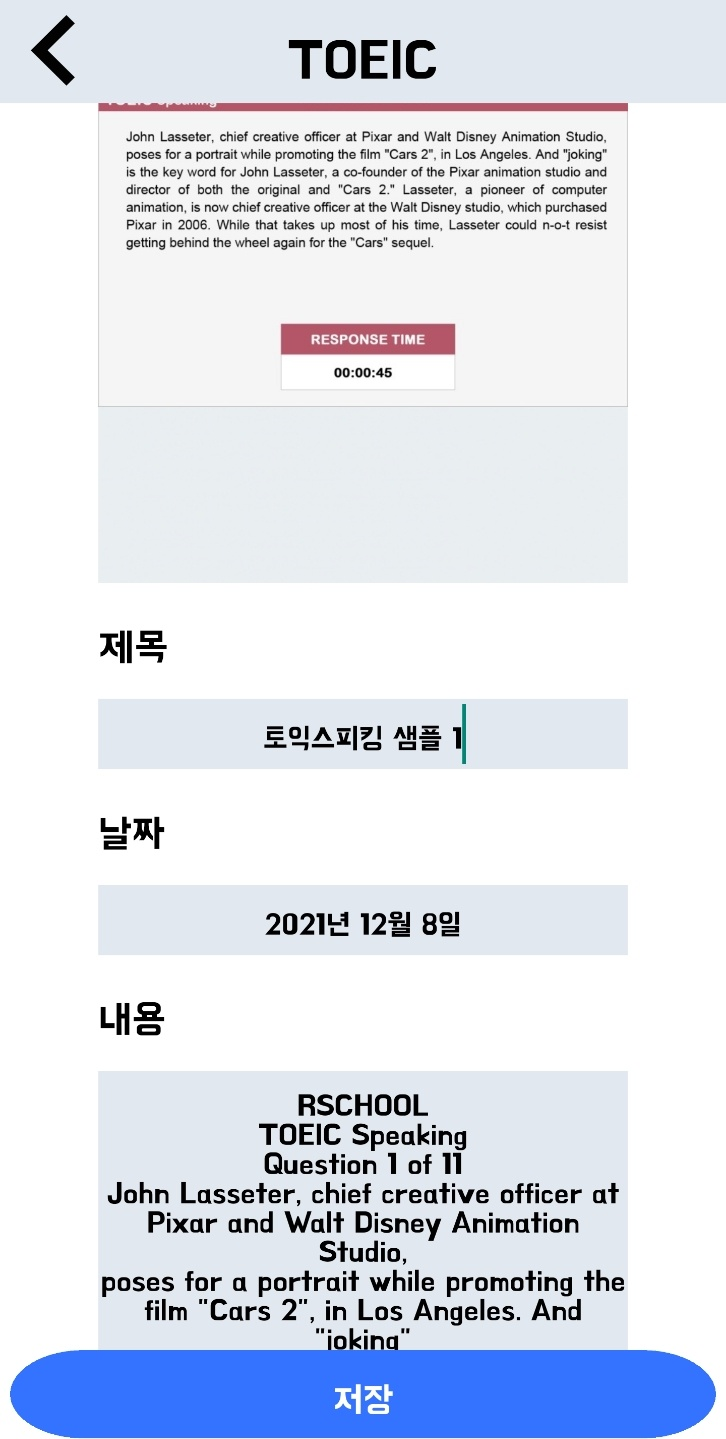
\includegraphics[width=5cm]{Images/app_note_toeic.png}
    \caption{Create a not for TOEIC subject}
\end{figure}

In the individual note page, the user can insert a picture and make use of OCR technology to scan the text inside and display it in a textbox. The following text blocks are about the title of the note and the date of it. The last textblock can be used to add or edit notes. The final button is used for saving the note. 


        \begin{figure}[htp]
    \centering
    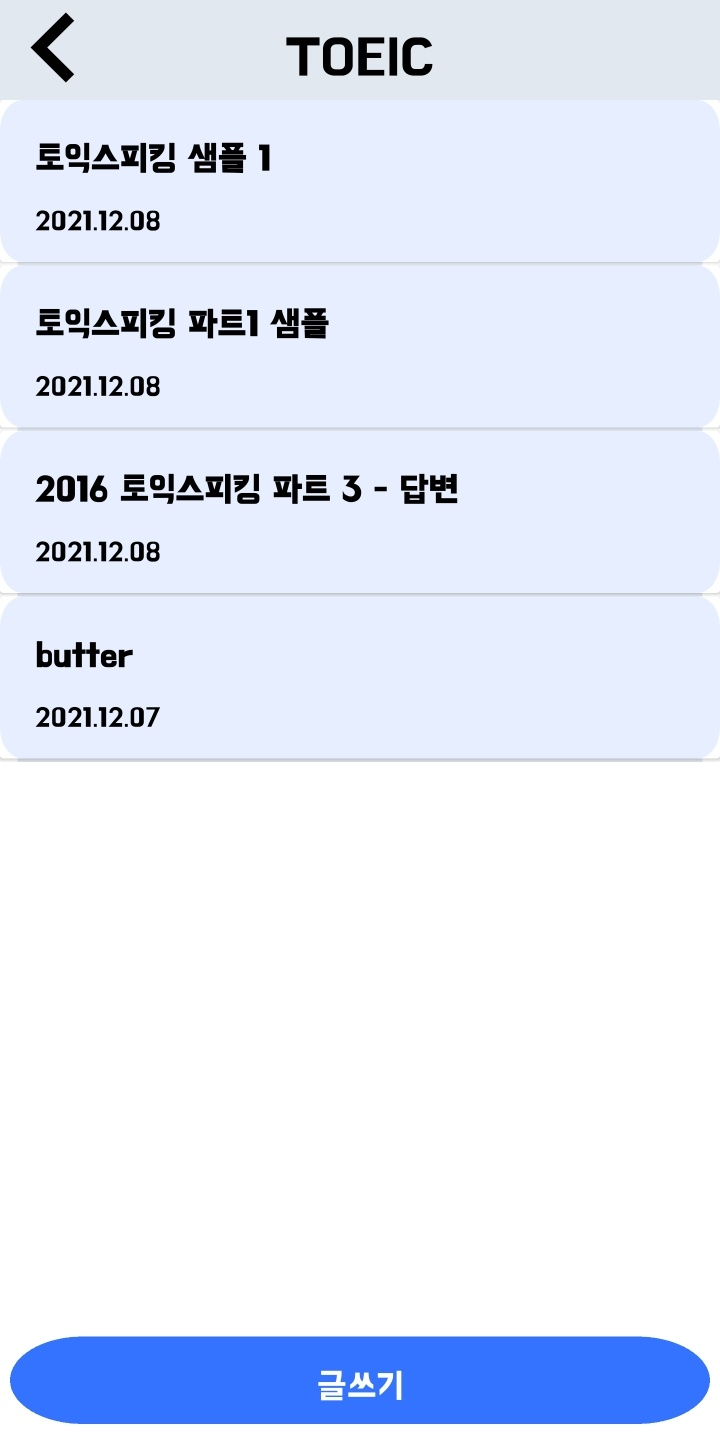
\includegraphics[width=5cm]{Images/app_note_newNote.png}
    \caption{Result of creating a new note}
\end{figure}

This function partly fulfils the requirement 4) Information Sharing Function (about study time) by allowing the user to create notes . When accessing the data in the backend, he is able to view notes from other students.\\
    
    \item \textit{Check notes}
    
            \begin{figure}[H]
    \centering
    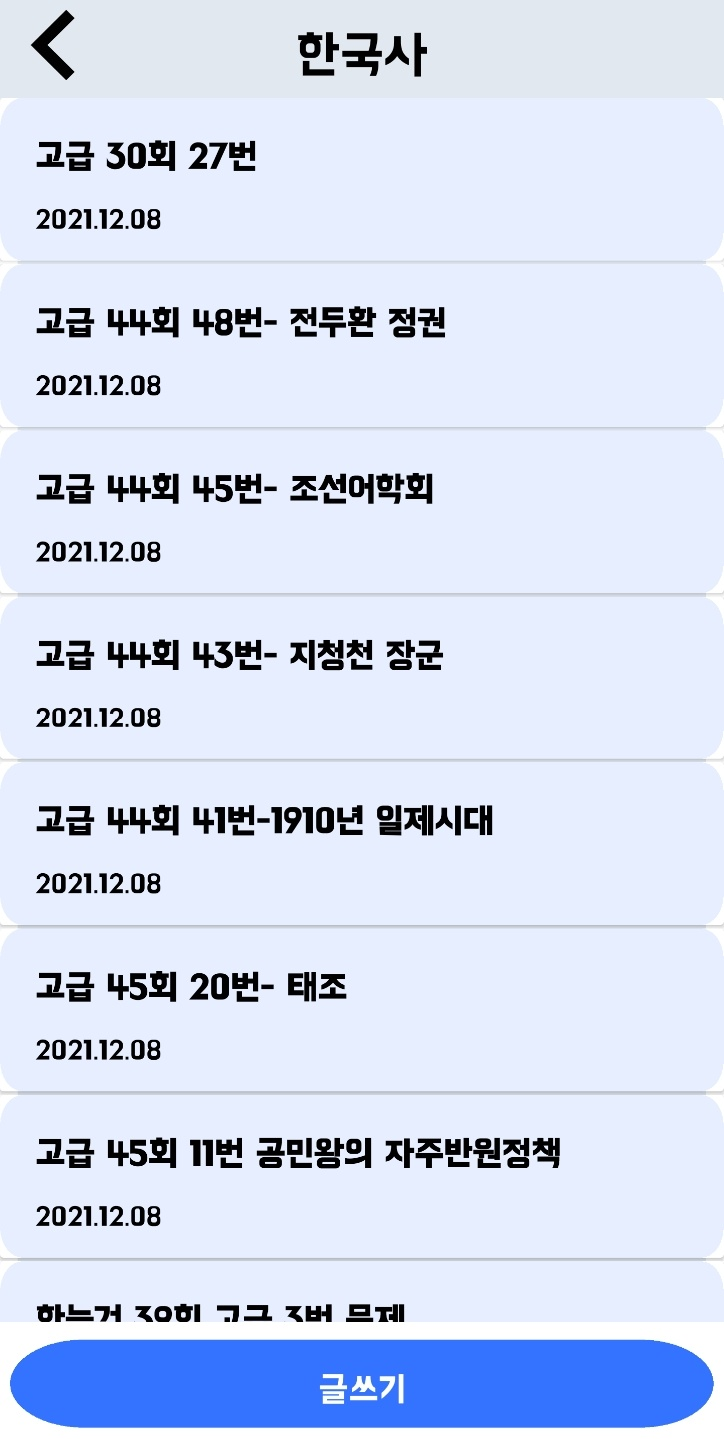
\includegraphics[width=5cm]{Images/app_note_notes.png}
    \caption{Overview on existing notes}
\end{figure}

When entering the note taking function and choosing a subject with at least one note, the existing notes are displayed and can be viewed or edited when clicking on them.

This function partly fulfils the requirements 4) Information Sharing Function (about study time) and 5) Group ranking and 6) Feedback by allowing the user to create notes for himself. When accessing the data in the backend, he is able to view notes from other students and get insights of his and their study progress.

    
\end{enumerate}

\end{enumerate}







\subsection{Use Case 2 - SKT NUGU AI Speaker}

\begin{enumerate}
    \item Installation
    
If the user purchases the NUGU Speaker, completes the speaker setup, and installs the NUGU application on the user's smartphone, the user is ready to use StudyBNB. If you press the menu in the upper left corner on the main screen of the NUGU application on your smartphone, StudyBNB exists in the Education/Childcare tab of the NUGU Play category.

\begin{figure}[htp]
    \centering
    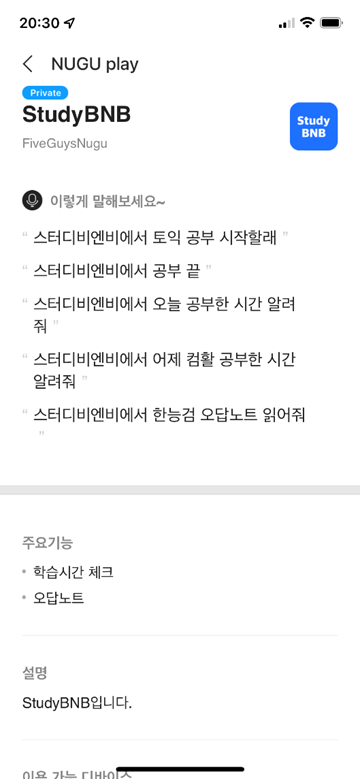
\includegraphics[width=5cm]{Images/NuguPlay_StudyBnB.png}
    \caption{Finding StudyBNB in the NUGU Play app}
\end{figure}

Users need to finish linking with StudyBNB service in this page. If users do not have a Studybnb account, users must first download the Studybnb Android application from the Google Play, register as a member, and then complete user settings. When this process is completed, users will be able to use StudyBNB's services in earnest.\\
    
    \item Starting Application
    
    There are two ways to call StudyBNB from NUGU Speaker.
    
    \begin{enumerate}
        \item Aria, start StudyBNB (아리아, 스터디비엔비 실행해줘) → Commands (like "start timer for TOEIC")
        
The advantage of using this method is that users can get more accurate results. However, there is a disadvantage that it takes a lot of time to execute the desired function because you must speak at least two commands.
        \item Aria, Commands (like "start timer for TOEIC") in StudyBNB (아리아, 스터디비엔비에서 토익 시간 체크 시작해줘)
        
Since the recognition rate of NUGU Speaker decreases significantly as the length of the command increases, the possibility that the speaker cannot properly recognize the user's speech increases if such a long command is used. But NUGU Speaker has a great AI Model, so it will learn commands continuously, and sooner or later, it will understand your commands easily. If the user has been using this application for a long time, the speaker will correctly understand this command and execute the function.\\

    \end{enumerate}

    
    
    \item Main Function
    \begin{enumerate}
        \item \textit{Start Timer}
        
        \begin{figure}[H]
    \centering
    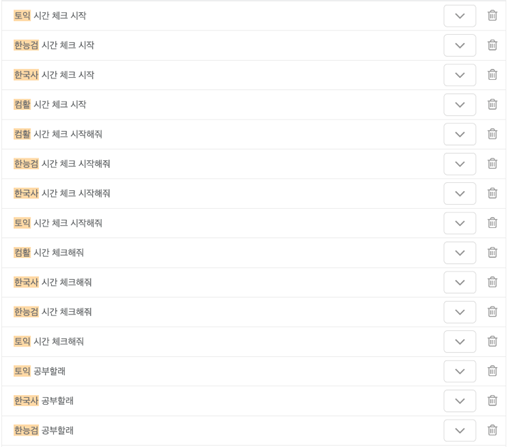
\includegraphics[width=8cm]{Images/nugu_start1.png}
\end{figure}
        \begin{figure}[H]
    \centering
    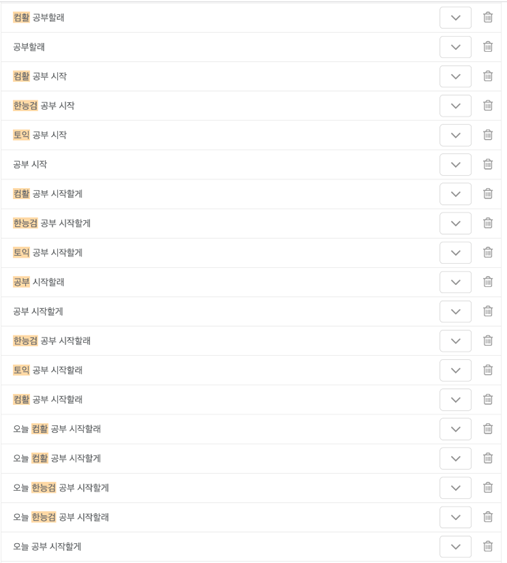
\includegraphics[width=8cm]{Images/nugu_start2.png}
\end{figure}
        \begin{figure}[H]
    \centering
    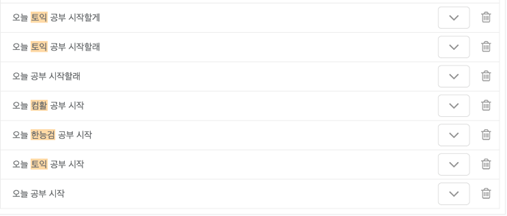
\includegraphics[width=8cm]{Images/nugu_start3.png}
    \caption{Actions to start timer}
\end{figure}
        
        Command: "Start timer for subject(including Korean History Exam, TOEIC, Computer Specialist in Spreadsheet and Database(CS))"
        
If you skip subject and execute the command, NUGU Speaker will ask you again about the subject information. If NUGU Speaker still does not receive the course information, the service will be terminated immediately because StudyBNB cannot process the command. When NUGU Speaker receives a normal command, it sends it to Flask Server and triggers timer function.

If the timer is running and the NUGU Speaker receives a command to start the timer, The Flask server will refuse to process the command because it cannot execute it. This is because it is impossible for one person to study several subjects at the same time.\\

        
        \item \textit{Finish Timer}
        
                \begin{figure}[H]
    \centering
    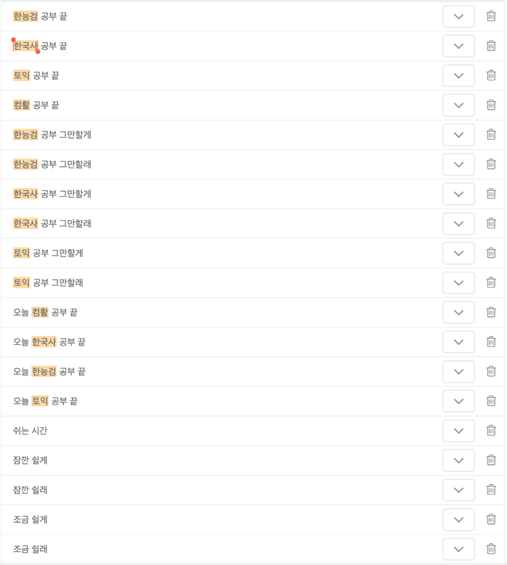
\includegraphics[width=8cm]{Images/nugu_finish1.png}
\end{figure}

        \begin{figure}[H]
    \centering
    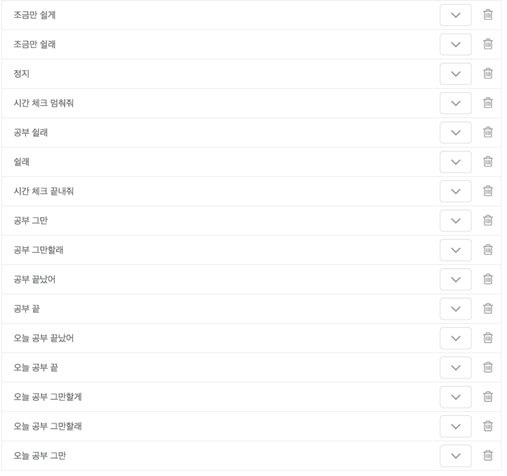
\includegraphics[width=8cm]{Images/nugu_finish2.png}
    \caption{Actions to finish timer}
\end{figure}

Command: "Finish timer" or "I need to rest"

Even if you omit the subject information, the Flask server works normally because it remembers which subject's timer you ran. When a speaker receives a command to finish studying, it will be sent to the Flask server to terminate the timer. If the timer has already expired and another timer termination request comes in, the Flask server will return an error code because it is a request that cannot be executed.\\

        
        \item \textit{Calculate study time for now}
        
                \begin{figure}[htp]
    \centering
    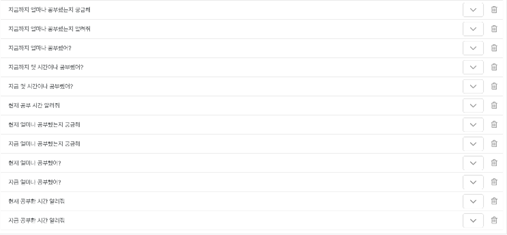
\includegraphics[width=8cm]{Images/nugu_calculate_now.png}
    \caption{Actions to calculate study time}
\end{figure}

Command: "Tell me what time I studied"

This is a function that can determine how much the user has studied while the timer is running. When the NUGU Speaker receives this command, the Flask server returns the hour, minute, and second of the currently studied time. If the timer is not turned on, the Flask server will return an error code because it cannot process this command.\\


        
        \item \textit{Calculate study time by subject or date}
        
                \begin{figure}[htp]
    \centering
    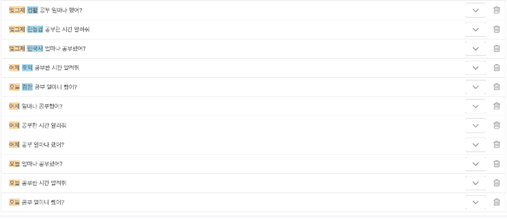
\includegraphics[width=8cm]{Images/nugu_calculate_subj.png}
    \caption{Actions to calculate study time for subject}
\end{figure}

Command: "How much did I study today" or "Tell me how long I studied the TOEIC yesterday"

This is a function that notifies the total study time or study time for a specific subject on a specific date. Since the date information is required, if this is not entered, the NUGU Speaker will ask the user to speak the date information again. Dates are supported only for today, yesterday, and yesterday. Because NUGU Speaker does not support date information flexibly, it is not easy to process date information that NUGU Speaker does not support. If subject information is not entered, the total study time for all subjects will be returned, and if inputted, the total study time for the entered subject will be returned. Also, if the timer is on, Flask server will count up to the current study time and return the total study time.\\


        \item \textit{Read Studynote}
        
                \begin{figure}[htp]
    \centering
    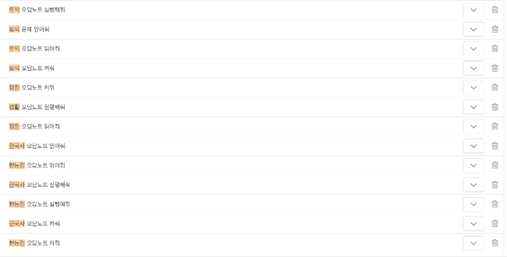
\includegraphics[width=8cm]{Images/nugu_readstudy.png}
    \caption{Actions to read notes}
\end{figure}
        
        Command: "Read wrong answer note of SUBJECT(like TOEIC, Korean History, CS)"
        
This is a function that reads the user's wrong question recorded in the wrong answer note. Before executing the function to read wrong answer notes in NUGU Speaker, information about the question must be recorded in the Firestore DB. If users take a picture of wrong answer problems in the incorrect answer note of StudyBNB Android Application, the text will be automatically extracted from the image through OCR function. If users take a picture of a problem in Korean, not in English, the performance is not good, so users have to edit the text themselves.

When users gives a command to NUGU Speaker, Subject information is essential because it is necessary to have subject information to call up the notes for incorrect answers. If the subject information is not entered, the Flask server will not be able to process the command, so the function will not be executed properly. If the command is processed normally, the Flask server will bring all the questions stored in the Firestore DB and deliver them to the NUGU Speaker. NUGU Speaker can't speak English well yet, but hopefully the quality will get better through collaboration with Amazon Alexa in the future.\\

        
        
        \item \textit{Get studymate's information}
        
        Command: "Is my studymate studying?" or "How much did my studymate study?"
        
To execute this function, you must first execute the matching function in StudyBNB Android Application. If the studymate is matched, the study information of user's studymate can be called from NUGU Speaker. User can check information such as how much his studymate has studied and whether he is currently studying. Currently, it is not implemented in the StudyBNB Android application and NUGU Speaker, but in the future, when a lot of users are gathered and data accumulates, the function will be implemented based on it.

    \end{enumerate}
\end{enumerate}

\section{Conclusions}

In this paper, the implementation of a study time checker service has been discussed to help students study more efficiently by not needing to check their smartphone too often. The resulted service makes use of an mobile app and the SKT NUGU AI Speaker to measure study time and create notes for popular exams like TOEIC. Clear benefits have been demonstrated by analysing user requirements, comparing existing software and making use of their disadvantages. 

When we first started our development plan, we planned to provide two paths: smartphone apps and AI speakers with two AI-based services: StudyMate and Note-taking.

However, due to limited development capabilities and time constraints, we had no choice but to produce slightly modified results from the initial plan. Among the many parts, the most regrettable thing is that the StudyMate function was not fully implemented in the app. If the service can be expanded as planned, the authors think that they can make a more functionally completed software.




\begin{thebibliography}{00}
\bibitem{b1} F. Jabr, "Why Your Brain Needs More Downtime", October 2013, https://www.scientificamerican.com/article/mental-downtime/
\bibitem{b2} H. Bae, “Review: How I study using a productivity app: Yeolpumta, September 2021, https://highschool.latimes.com/la-canada-high-school/review-how-i-study-using-a-productivity-app-yeolpumta/ 
\bibitem{b3} Study International Staff, “Studying at home? Here are the best productivity apps to check out”, March 2020, https://www.studyinternational.com/news/5-apps-focus-study-home/
\bibitem{b4} K. Udoagwu, “How to Carry Out a Requirements Analysis”, February 2021, https://www.wrike.com/blog/how-carry-out-requirements-analysis/\#What-is-the-requirements-analysis-process
\bibitem{b5} M. Jimin, “외워야 할 것 있다면 잠들기 전 집중하세요”, April 2019, https://m.health.chosun.com/svc/news\_view.html?contid=2019041801775

\end{thebibliography}
\vspace{12pt}


\end{document}
